% Target ≤20 pages. Prefer images over text. Keep captions concise.
\documentclass[12pt,letterpaper]{article}

% Load custom portfolio style
\usepackage{styles/portfolio}

% ---------------------------------------------------------------------------- %
%                                 NEW MATH DEF                                 %
% ---------------------------------------------------------------------------- %

\usepackage{amsmath,amsfonts,bm}

% Mark sections of captions for referring to divisions of figures
\newcommand{\figleft}{{\em (Left)}}
\newcommand{\figcenter}{{\em (Center)}}
\newcommand{\figright}{{\em (Right)}}
\newcommand{\figtop}{{\em (Top)}}
\newcommand{\figbottom}{{\em (Bottom)}}
\newcommand{\captiona}{{\em (a)}}
\newcommand{\captionb}{{\em (b)}}
\newcommand{\captionc}{{\em (c)}}
\newcommand{\captiond}{{\em (d)}}

% Highlight a newly defined term
\newcommand{\newterm}[1]{{\bf #1}}


\def\figref#1{figure~\ref{#1}}
\def\Figref#1{Figure~\ref{#1}}
\def\twofigref#1#2{figures \ref{#1} and \ref{#2}}
\def\quadfigref#1#2#3#4{figures \ref{#1}, \ref{#2}, \ref{#3} and \ref{#4}}
\def\secref#1{section~\ref{#1}}
\def\Secref#1{Section~\ref{#1}}
\def\twosecrefs#1#2{sections \ref{#1} and \ref{#2}}
\def\secrefs#1#2#3{sections \ref{#1}, \ref{#2} and \ref{#3}}
\def\eqref#1{equation~\ref{#1}}
\def\Eqref#1{Equation~\ref{#1}}
\def\plaineqref#1{\ref{#1}}
\def\chapref#1{chapter~\ref{#1}}
\def\Chapref#1{Chapter~\ref{#1}}
\def\rangechapref#1#2{chapters\ref{#1}--\ref{#2}}
\def\algref#1{algorithm~\ref{#1}}
\def\Algref#1{Algorithm~\ref{#1}}
\def\twoalgref#1#2{algorithms \ref{#1} and \ref{#2}}
\def\Twoalgref#1#2{Algorithms \ref{#1} and \ref{#2}}
\def\partref#1{part~\ref{#1}}
\def\Partref#1{Part~\ref{#1}}
\def\twopartref#1#2{parts \ref{#1} and \ref{#2}}

\def\ceil#1{\lceil #1 \rceil}
\def\floor#1{\lfloor #1 \rfloor}
\def\1{\bm{1}}
\newcommand{\train}{\mathcal{D}}
\newcommand{\valid}{\mathcal{D_{\mathrm{valid}}}}
\newcommand{\test}{\mathcal{D_{\mathrm{test}}}}

\def\eps{{\epsilon}}

% Random variables
\def\reta{{\textnormal{$\eta$}}}
\def\ra{{\textnormal{a}}}
\def\rb{{\textnormal{b}}}
\def\rc{{\textnormal{c}}}
\def\rd{{\textnormal{d}}}
\def\re{{\textnormal{e}}}
\def\rf{{\textnormal{f}}}
\def\rg{{\textnormal{g}}}
\def\rh{{\textnormal{h}}}
\def\ri{{\textnormal{i}}}
\def\rj{{\textnormal{j}}}
\def\rk{{\textnormal{k}}}
\def\rl{{\textnormal{l}}}
% rm is already a command
\def\rn{{\textnormal{n}}}
\def\ro{{\textnormal{o}}}
\def\rp{{\textnormal{p}}}
\def\rq{{\textnormal{q}}}
\def\rr{{\textnormal{r}}}
\def\rs{{\textnormal{s}}}
\def\rt{{\textnormal{t}}}
\def\ru{{\textnormal{u}}}
\def\rv{{\textnormal{v}}}
\def\rw{{\textnormal{w}}}
\def\rx{{\textnormal{x}}}
\def\ry{{\textnormal{y}}}
\def\rz{{\textnormal{z}}}

% Random vectors
\def\rvepsilon{{\mathbf{\epsilon}}}
\def\rvtheta{{\mathbf{\theta}}}
\def\rva{{\mathbf{a}}}
\def\rvb{{\mathbf{b}}}
\def\rvc{{\mathbf{c}}}
\def\rvd{{\mathbf{d}}}
\def\rve{{\mathbf{e}}}
\def\rvf{{\mathbf{f}}}
\def\rvg{{\mathbf{g}}}
\def\rvh{{\mathbf{h}}}
\def\rvu{{\mathbf{i}}}
\def\rvj{{\mathbf{j}}}
\def\rvk{{\mathbf{k}}}
\def\rvl{{\mathbf{l}}}
\def\rvm{{\mathbf{m}}}
\def\rvn{{\mathbf{n}}}
\def\rvo{{\mathbf{o}}}
\def\rvp{{\mathbf{p}}}
\def\rvq{{\mathbf{q}}}
\def\rvr{{\mathbf{r}}}
\def\rvs{{\mathbf{s}}}
\def\rvt{{\mathbf{t}}}
\def\rvu{{\mathbf{u}}}
\def\rvv{{\mathbf{v}}}
\def\rvw{{\mathbf{w}}}
\def\rvx{{\mathbf{x}}}
\def\rvy{{\mathbf{y}}}
\def\rvz{{\mathbf{z}}}

% Elements of random vectors
\def\erva{{\textnormal{a}}}
\def\ervb{{\textnormal{b}}}
\def\ervc{{\textnormal{c}}}
\def\ervd{{\textnormal{d}}}
\def\erve{{\textnormal{e}}}
\def\ervf{{\textnormal{f}}}
\def\ervg{{\textnormal{g}}}
\def\ervh{{\textnormal{h}}}
\def\ervi{{\textnormal{i}}}
\def\ervj{{\textnormal{j}}}
\def\ervk{{\textnormal{k}}}
\def\ervl{{\textnormal{l}}}
\def\ervm{{\textnormal{m}}}
\def\ervn{{\textnormal{n}}}
\def\ervo{{\textnormal{o}}}
\def\ervp{{\textnormal{p}}}
\def\ervq{{\textnormal{q}}}
\def\ervr{{\textnormal{r}}}
\def\ervs{{\textnormal{s}}}
\def\ervt{{\textnormal{t}}}
\def\ervu{{\textnormal{u}}}
\def\ervv{{\textnormal{v}}}
\def\ervw{{\textnormal{w}}}
\def\ervx{{\textnormal{x}}}
\def\ervy{{\textnormal{y}}}
\def\ervz{{\textnormal{z}}}

% Random matrices
\def\rmA{{\mathbf{A}}}
\def\rmB{{\mathbf{B}}}
\def\rmC{{\mathbf{C}}}
\def\rmD{{\mathbf{D}}}
\def\rmE{{\mathbf{E}}}
\def\rmF{{\mathbf{F}}}
\def\rmG{{\mathbf{G}}}
\def\rmH{{\mathbf{H}}}
\def\rmI{{\mathbf{I}}}
\def\rmJ{{\mathbf{J}}}
\def\rmK{{\mathbf{K}}}
\def\rmL{{\mathbf{L}}}
\def\rmM{{\mathbf{M}}}
\def\rmN{{\mathbf{N}}}
\def\rmO{{\mathbf{O}}}
\def\rmP{{\mathbf{P}}}
\def\rmQ{{\mathbf{Q}}}
\def\rmR{{\mathbf{R}}}
\def\rmS{{\mathbf{S}}}
\def\rmT{{\mathbf{T}}}
\def\rmU{{\mathbf{U}}}
\def\rmV{{\mathbf{V}}}
\def\rmW{{\mathbf{W}}}
\def\rmX{{\mathbf{X}}}
\def\rmY{{\mathbf{Y}}}
\def\rmZ{{\mathbf{Z}}}

% Elements of random matrices
\def\ermA{{\textnormal{A}}}
\def\ermB{{\textnormal{B}}}
\def\ermC{{\textnormal{C}}}
\def\ermD{{\textnormal{D}}}
\def\ermE{{\textnormal{E}}}
\def\ermF{{\textnormal{F}}}
\def\ermG{{\textnormal{G}}}
\def\ermH{{\textnormal{H}}}
\def\ermI{{\textnormal{I}}}
\def\ermJ{{\textnormal{J}}}
\def\ermK{{\textnormal{K}}}
\def\ermL{{\textnormal{L}}}
\def\ermM{{\textnormal{M}}}
\def\ermN{{\textnormal{N}}}
\def\ermO{{\textnormal{O}}}
\def\ermP{{\textnormal{P}}}
\def\ermQ{{\textnormal{Q}}}
\def\ermR{{\textnormal{R}}}
\def\ermS{{\textnormal{S}}}
\def\ermT{{\textnormal{T}}}
\def\ermU{{\textnormal{U}}}
\def\ermV{{\textnormal{V}}}
\def\ermW{{\textnormal{W}}}
\def\ermX{{\textnormal{X}}}
\def\ermY{{\textnormal{Y}}}
\def\ermZ{{\textnormal{Z}}}

% Vectors
\def\vzero{{\bm{0}}}
\def\vone{{\bm{1}}}
\def\vmu{{\bm{\mu}}}
\def\vtheta{{\bm{\theta}}}
\def\va{{\bm{a}}}
\def\vb{{\bm{b}}}
\def\vc{{\bm{c}}}
\def\vd{{\bm{d}}}
\def\ve{{\bm{e}}}
\def\vf{{\bm{f}}}
\def\vg{{\bm{g}}}
\def\vh{{\bm{h}}}
\def\vi{{\bm{i}}}
\def\vj{{\bm{j}}}
\def\vk{{\bm{k}}}
\def\vl{{\bm{l}}}
\def\vm{{\bm{m}}}
\def\vn{{\bm{n}}}
\def\vo{{\bm{o}}}
\def\vp{{\bm{p}}}
\def\vq{{\bm{q}}}
\def\vr{{\bm{r}}}
\def\vs{{\bm{s}}}
\def\vt{{\bm{t}}}
\def\vu{{\bm{u}}}
\def\vv{{\bm{v}}}
\def\vw{{\bm{w}}}
\def\vx{{\bm{x}}}
\def\vy{{\bm{y}}}
\def\vz{{\bm{z}}}
\def\vomega{{\bm{\omega}}}

% Elements of vectors
\def\evalpha{{\alpha}}
\def\evbeta{{\beta}}
\def\evepsilon{{\epsilon}}
\def\evlambda{{\lambda}}
\def\evomega{{\omega}}
\def\evmu{{\mu}}
\def\evpsi{{\psi}}
\def\evsigma{{\sigma}}
\def\evtheta{{\theta}}
\def\eva{{a}}
\def\evb{{b}}
\def\evc{{c}}
\def\evd{{d}}
\def\eve{{e}}
\def\evf{{f}}
\def\evg{{g}}
\def\evh{{h}}
\def\evi{{i}}
\def\evj{{j}}
\def\evk{{k}}
\def\evl{{l}}
\def\evm{{m}}
\def\evn{{n}}
\def\evo{{o}}
\def\evp{{p}}
\def\evq{{q}}
\def\evr{{r}}
\def\evs{{s}}
\def\evt{{t}}
\def\evu{{u}}
\def\evv{{v}}
\def\evw{{w}}
\def\evx{{x}}
\def\evy{{y}}
\def\evz{{z}}
\def\evomega{{\omega}}

% Matrix
\def\mA{{\bm{A}}}
\def\mB{{\bm{B}}}
\def\mC{{\bm{C}}}
\def\mD{{\bm{D}}}
\def\mE{{\bm{E}}}
\def\mF{{\bm{F}}}
\def\mG{{\bm{G}}}
\def\mH{{\bm{H}}}
\def\mI{{\bm{I}}}
\def\mJ{{\bm{J}}}
\def\mK{{\bm{K}}}
\def\mL{{\bm{L}}}
\def\mM{{\bm{M}}}
\def\mN{{\bm{N}}}
\def\mO{{\bm{O}}}
\def\mP{{\bm{P}}}
\def\mQ{{\bm{Q}}}
\def\mR{{\bm{R}}}
\def\mS{{\bm{S}}}
\def\mT{{\bm{T}}}
\def\mU{{\bm{U}}}
\def\mV{{\bm{V}}}
\def\mW{{\bm{W}}}
\def\mX{{\bm{X}}}
\def\mY{{\bm{Y}}}
\def\mZ{{\bm{Z}}}
\def\mBeta{{\bm{\beta}}}
\def\mPhi{{\bm{\Phi}}}
\def\mLambda{{\bm{\Lambda}}}
\def\mSigma{{\bm{\Sigma}}}
\def\mOmega{{\bm{\Omega}}}

% Tensor
\DeclareMathAlphabet{\mathsfit}{\encodingdefault}{\sfdefault}{m}{sl}
\SetMathAlphabet{\mathsfit}{bold}{\encodingdefault}{\sfdefault}{bx}{n}
\newcommand{\tens}[1]{\bm{\mathsfit{#1}}}
\def\tA{{\tens{A}}}
\def\tB{{\tens{B}}}
\def\tC{{\tens{C}}}
\def\tD{{\tens{D}}}
\def\tE{{\tens{E}}}
\def\tF{{\tens{F}}}
\def\tG{{\tens{G}}}
\def\tH{{\tens{H}}}
\def\tI{{\tens{I}}}
\def\tJ{{\tens{J}}}
\def\tK{{\tens{K}}}
\def\tL{{\tens{L}}}
\def\tM{{\tens{M}}}
\def\tN{{\tens{N}}}
\def\tO{{\tens{O}}}
\def\tP{{\tens{P}}}
\def\tQ{{\tens{Q}}}
\def\tR{{\tens{R}}}
\def\tS{{\tens{S}}}
\def\tT{{\tens{T}}}
\def\tU{{\tens{U}}}
\def\tV{{\tens{V}}}
\def\tW{{\tens{W}}}
\def\tX{{\tens{X}}}
\def\tY{{\tens{Y}}}
\def\tZ{{\tens{Z}}}


% Graph
\def\gA{{\mathcal{A}}}
\def\gB{{\mathcal{B}}}
\def\gC{{\mathcal{C}}}
\def\gD{{\mathcal{D}}}
\def\gE{{\mathcal{E}}}
\def\gF{{\mathcal{F}}}
\def\gG{{\mathcal{G}}}
\def\gH{{\mathcal{H}}}
\def\gI{{\mathcal{I}}}
\def\gJ{{\mathcal{J}}}
\def\gK{{\mathcal{K}}}
\def\gL{{\mathcal{L}}}
\def\gM{{\mathcal{M}}}
\def\gN{{\mathcal{N}}}
\def\gO{{\mathcal{O}}}
\def\gP{{\mathcal{P}}}
\def\gQ{{\mathcal{Q}}}
\def\gR{{\mathcal{R}}}
\def\gS{{\mathcal{S}}}
\def\gT{{\mathcal{T}}}
\def\gU{{\mathcal{U}}}
\def\gV{{\mathcal{V}}}
\def\gW{{\mathcal{W}}}
\def\gX{{\mathcal{X}}}
\def\gY{{\mathcal{Y}}}
\def\gZ{{\mathcal{Z}}}
\def\gOne{{\mathcal{1}}}

% Sets
\def\sA{{\mathbb{A}}}
\def\sB{{\mathbb{B}}}
\def\sC{{\mathbb{C}}}
\def\sD{{\mathbb{D}}}
% Don't use a set called E, because this would be the same as our symbol
% for expectation.
\def\sE{{\mathbb{E}}} % force for edge set
\def\sF{{\mathbb{F}}}
\def\sG{{\mathbb{G}}}
\def\sH{{\mathbb{H}}}
\def\sI{{\mathbb{I}}}
\def\sJ{{\mathbb{J}}}
\def\sK{{\mathbb{K}}}
\def\sL{{\mathbb{L}}}
\def\sM{{\mathbb{M}}}
\def\sN{{\mathbb{N}}}
\def\sO{{\mathbb{O}}}
\def\sP{{\mathbb{P}}}
\def\sQ{{\mathbb{Q}}}
\def\sR{{\mathbb{R}}}
\def\sS{{\mathbb{S}}}
\def\sT{{\mathbb{T}}}
\def\sU{{\mathbb{U}}}
\def\sV{{\mathbb{V}}}
\def\sW{{\mathbb{W}}}
\def\sX{{\mathbb{X}}}
\def\sY{{\mathbb{Y}}}
\def\sZ{{\mathbb{Z}}}

% Entries of a matrix
\def\emLambda{{\Lambda}}
\def\emA{{A}}
\def\emB{{B}}
\def\emC{{C}}
\def\emD{{D}}
\def\emE{{E}}
\def\emF{{F}}
\def\emG{{G}}
\def\emH{{H}}
\def\emI{{I}}
\def\emJ{{J}}
\def\emK{{K}}
\def\emL{{L}}
\def\emM{{M}}
\def\emN{{N}}
\def\emO{{O}}
\def\emP{{P}}
\def\emQ{{Q}}
\def\emR{{R}}
\def\emS{{S}}
\def\emT{{T}}
\def\emU{{U}}
\def\emV{{V}}
\def\emW{{W}}
\def\emX{{X}}
\def\emY{{Y}}
\def\emZ{{Z}}
\def\emSigma{{\Sigma}}

% entries of a tensor
% Same font as tensor, without \bm wrapper
\newcommand{\etens}[1]{\mathsfit{#1}}
\def\etLambda{{\etens{\Lambda}}}
\def\etA{{\etens{A}}}
\def\etB{{\etens{B}}}
\def\etC{{\etens{C}}}
\def\etD{{\etens{D}}}
\def\etE{{\etens{E}}}
\def\etF{{\etens{F}}}
\def\etG{{\etens{G}}}
\def\etH{{\etens{H}}}
\def\etI{{\etens{I}}}
\def\etJ{{\etens{J}}}
\def\etK{{\etens{K}}}
\def\etL{{\etens{L}}}
\def\etM{{\etens{M}}}
\def\etN{{\etens{N}}}
\def\etO{{\etens{O}}}
\def\etP{{\etens{P}}}
\def\etQ{{\etens{Q}}}
\def\etR{{\etens{R}}}
\def\etS{{\etens{S}}}
\def\etT{{\etens{T}}}
\def\etU{{\etens{U}}}
\def\etV{{\etens{V}}}
\def\etW{{\etens{W}}}
\def\etX{{\etens{X}}}
\def\etY{{\etens{Y}}}
\def\etZ{{\etens{Z}}}

% The true underlying data generating distribution
\newcommand{\pdata}{p_{\rm{data}}}
% The empirical distribution defined by the training set
\newcommand{\ptrain}{\hat{p}_{\rm{data}}}
\newcommand{\Ptrain}{\hat{P}_{\rm{data}}}
% The model distribution
\newcommand{\pmodel}{p_{\rm{model}}}
\newcommand{\Pmodel}{P_{\rm{model}}}
\newcommand{\ptildemodel}{\tilde{p}_{\rm{model}}}
% Stochastic autoencoder distributions
\newcommand{\pencode}{p_{\rm{encoder}}}
\newcommand{\pdecode}{p_{\rm{decoder}}}
\newcommand{\precons}{p_{\rm{reconstruct}}}

\providecommand{\laplace}{\mathrm{Laplace}} % Laplace distribution

\newcommand{\E}{\mathbb{E}}
\newcommand{\Ls}{\mathcal{L}}
\newcommand{\R}{\mathbb{R}}
\newcommand{\emp}{\tilde{p}}
\newcommand{\lr}{\alpha}
\newcommand{\reg}{\lambda}
\newcommand{\rect}{\mathrm{rectifier}}
\newcommand{\softmax}{\mathrm{softmax}}
\newcommand{\sigmoid}{\sigma}
\newcommand{\softplus}{\zeta}
\newcommand{\KL}{D_{\mathrm{KL}}}
\newcommand{\Var}{\mathrm{Var}}
\newcommand{\standarderror}{\mathrm{SE}}
\newcommand{\Cov}{\mathrm{Cov}}
% Wolfram Mathworld says $L^2$ is for function spaces and $\ell^2$ is for vectors
% But then they seem to use $L^2$ for vectors throughout the site, and so does
% wikipedia.
\newcommand{\normlzero}{L^0}
\newcommand{\normlone}{L^1}
\newcommand{\normltwo}{L^2}
\newcommand{\normlp}{L^p}
\newcommand{\normmax}{L^\infty}

\newcommand{\parents}{Pa} % See usage in notation.tex. Chosen to match Daphne's book.

\DeclareMathOperator*{\argmax}{arg\,max}
\DeclareMathOperator*{\argmin}{arg\,min}

\DeclareMathOperator{\sign}{sign}
\DeclareMathOperator{\Tr}{Tr}
\let\ab\allowbreak
\newcommand{\s}[1]{\textcolor{gray}{\scriptsize{±#1}}}
\newcommand{\lb}[1]{\textbf{#1}}
\newcommand{\gb}[1]{\textbf{\underline{#1}}}
\usetikzlibrary{arrows.meta,positioning,calc,decorations.pathreplacing}

% ============================================================================
% PDF METADATA
% ============================================================================
\hypersetup{
  pdftitle={Juntang Wang - Academic Portfolio},
  pdfauthor={Juntang Wang},
  pdfsubject={Portfolio of Applied Mathematics, Computer Science, and AI Research},
  pdfkeywords={Machine Learning, Applied Mathematics, Computational Science, Data Science, Research, Duke}
}

\begin{document}

% ============================================================================
% COVER PAGE
% ============================================================================
\thispagestyle{nopagenumber}
% ============================================================================
% COVER PAGE
% ============================================================================

\begin{center}

% Name
{\Huge\bfseries Juntang Wang}

\vspace{0.5em}

% Program & Affiliation
{\Large Duke Kunshan University \& Duke University}\\[0.3em]
{\large B.S. Applied Math \& Computational Science; Computer Science Track}\\[-0.2em]
{\small Class of 2026}

\vspace{1em}

% Contact Information
\begin{tabular}{c}
  \faIcon{envelope} \href{mailto:jw853@duke.edu}{jw853@duke.edu} \\[0.2em]
  \faIcon{github} \href{https://github.com/qqgjyx}{github.com/qqgjyx} \\[0.2em]
  \faIcon{globe} \href{https://www.qqgjyx.com}{www.qqgjyx.com} \\[0.2em]
  \faIcon{map-marker-alt} Kunshan, CN \textbullet{} Durham, USA
\end{tabular}

\vspace{1.5em}

% Two-column layout: Tagline + Headshot
\begin{minipage}[t]{0.6\textwidth}
  \raggedright
  \vspace{0pt}
  
  \textcolor{Accent}{\rule{\linewidth}{2pt}}
  
  \vspace{0.5em}
  
  {\large\textit{Bridging AI, mathematics, and biomedical modeling through computational design and visualization.}}
  
  % Epigraph (Marcus Aurelius) with adaptation summarizing work
  \vspace{0.8em}
  {\small\begin{quote}\itshape
  “The impediment to action advances action. What stands in the way becomes the way.”\\
  {\normalfont\textcolor{LightGray}{— Marcus Aurelius, Meditations 5.20}}\\[0.3em]
  \textcolor{TextGray}{Turning obstacles into methods across AI, math, and biomedicine.}
  \end{quote}}
  
  \vspace{0.35em}
  
  \textcolor{Accent}{\rule{\linewidth}{2pt}}
  
\end{minipage}\hfill
\begin{minipage}[t]{0.35\textwidth}
  \raggedleft
  \vspace{0pt}
  
  % Headshot
  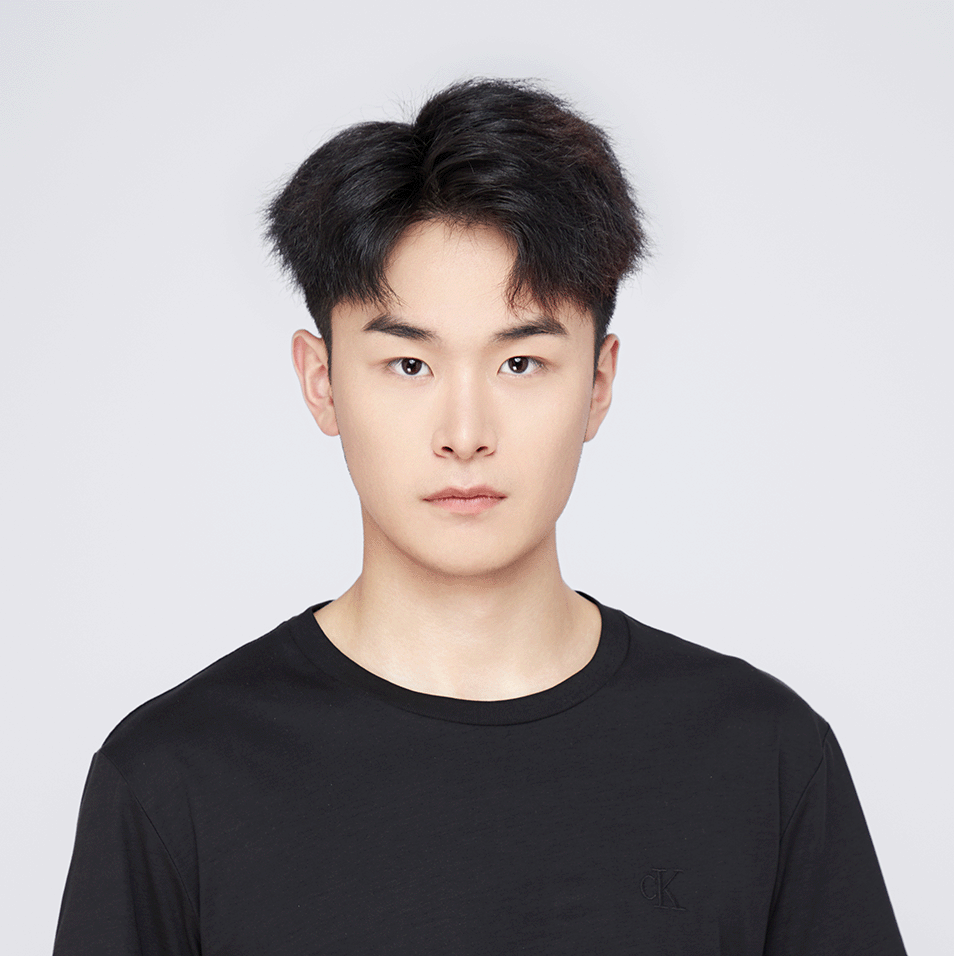
\includegraphics[width=0.76\linewidth]{assets/headshot.jpg}
  
  \vspace{0.5em}
  
  % QR code to website
  \qr{https://www.qqgjyx.com}
  
  \vspace{0.2em}
  
  {\footnotesize\textcolor{LightGray}{\textsc{Website}}}
\end{minipage}

\vspace{2.4em}

% Brief Introduction
\begin{minipage}{0.85\textwidth}
  \raggedright
  
  \section*{About This Portfolio}
  
  This portfolio showcases my work at the intersection of artificial intelligence, applied mathematics, and computational science. It includes research contributions under peer review at top-tier conferences (ICLR, BICS), open-source software tools with 600+ GitHub stars, teaching experience, and computational modeling projects.
  
  \vspace{0.5em}
  
  Each project demonstrates technical depth, practical impact, and creative problem-solving across machine learning, systems design, and computational modeling.
  
\end{minipage}

\end{center}


\newpage

% ============================================================================
% TABLE OF CONTENTS
% ============================================================================
\setcounter{tocdepth}{2}
\tableofcontents
\newpage

% ============================================================================
% RESEARCH PROJECTS (6–8 pages)
% ============================================================================
% ============================================================================
% RESEARCH PROJECTS
% ============================================================================

\section*{Research Projects}
\addcontentsline{toc}{section}{Research Projects}

% ---------------------------------------------------------------------------
% PROJECT 4: GraMixC
% ---------------------------------------------------------------------------

\addcontentsline{toc}{subsection}{Mixing Configurations for Downstream Prediction (ICLR 2026 under review)}
\ProjectEntry
{Mixing Configurations for Downstream Prediction}
{First Author, Research Assistant with Prof. Shixin Xu}
{Python, PyTorch, Unsupervised Learning}
{
  \bitem{Proposed GraMixC: a configuration\,–\,mixing module that fuses unsupervised ``configurations'' with task predictors for label\,–\,efficient downstream performance.}
  \bitem{Defined configuration extraction and mixing objectives, and integrated them with linear probing / 3LP predictors without changing the backbone.}
  \bitem{Validated on DSNI regression (pH/temperature) and image benchmarks; figures show attention maps, lineage diagrams, and quantitative gains.}
  \bitem{Ablation demonstrates incremental mixing (GMC) outperforms static concatenation (GC).}
  \bitem{Co-authored with Hao Wu, Runkun Guo, Yihan Wang, Dongmian Zou, and Prof. Shixin Xu; under ICLR 2026 review.}
}
{assets/1004_gramixc/framework.png}
{\extlink{https://arxiv.org/abs/2510.19248}{arXiv preprint}}
{\badge{Unsupervised Learning} \badge{ICLR under review}}


\textbf{Technical Highlights:}
This project tackles the challenge of learning meaningful representations from unlabeled data by mixing configurations in a learned latent space. The key innovation is a training objective that encourages the model to predict properties of mixed configurations based on the mixing coefficients and component configurations.

\begin{figure}[ht]
  \centering
  \subcaptionbox{Configurations\label{fig:cifar10_linage}}{
    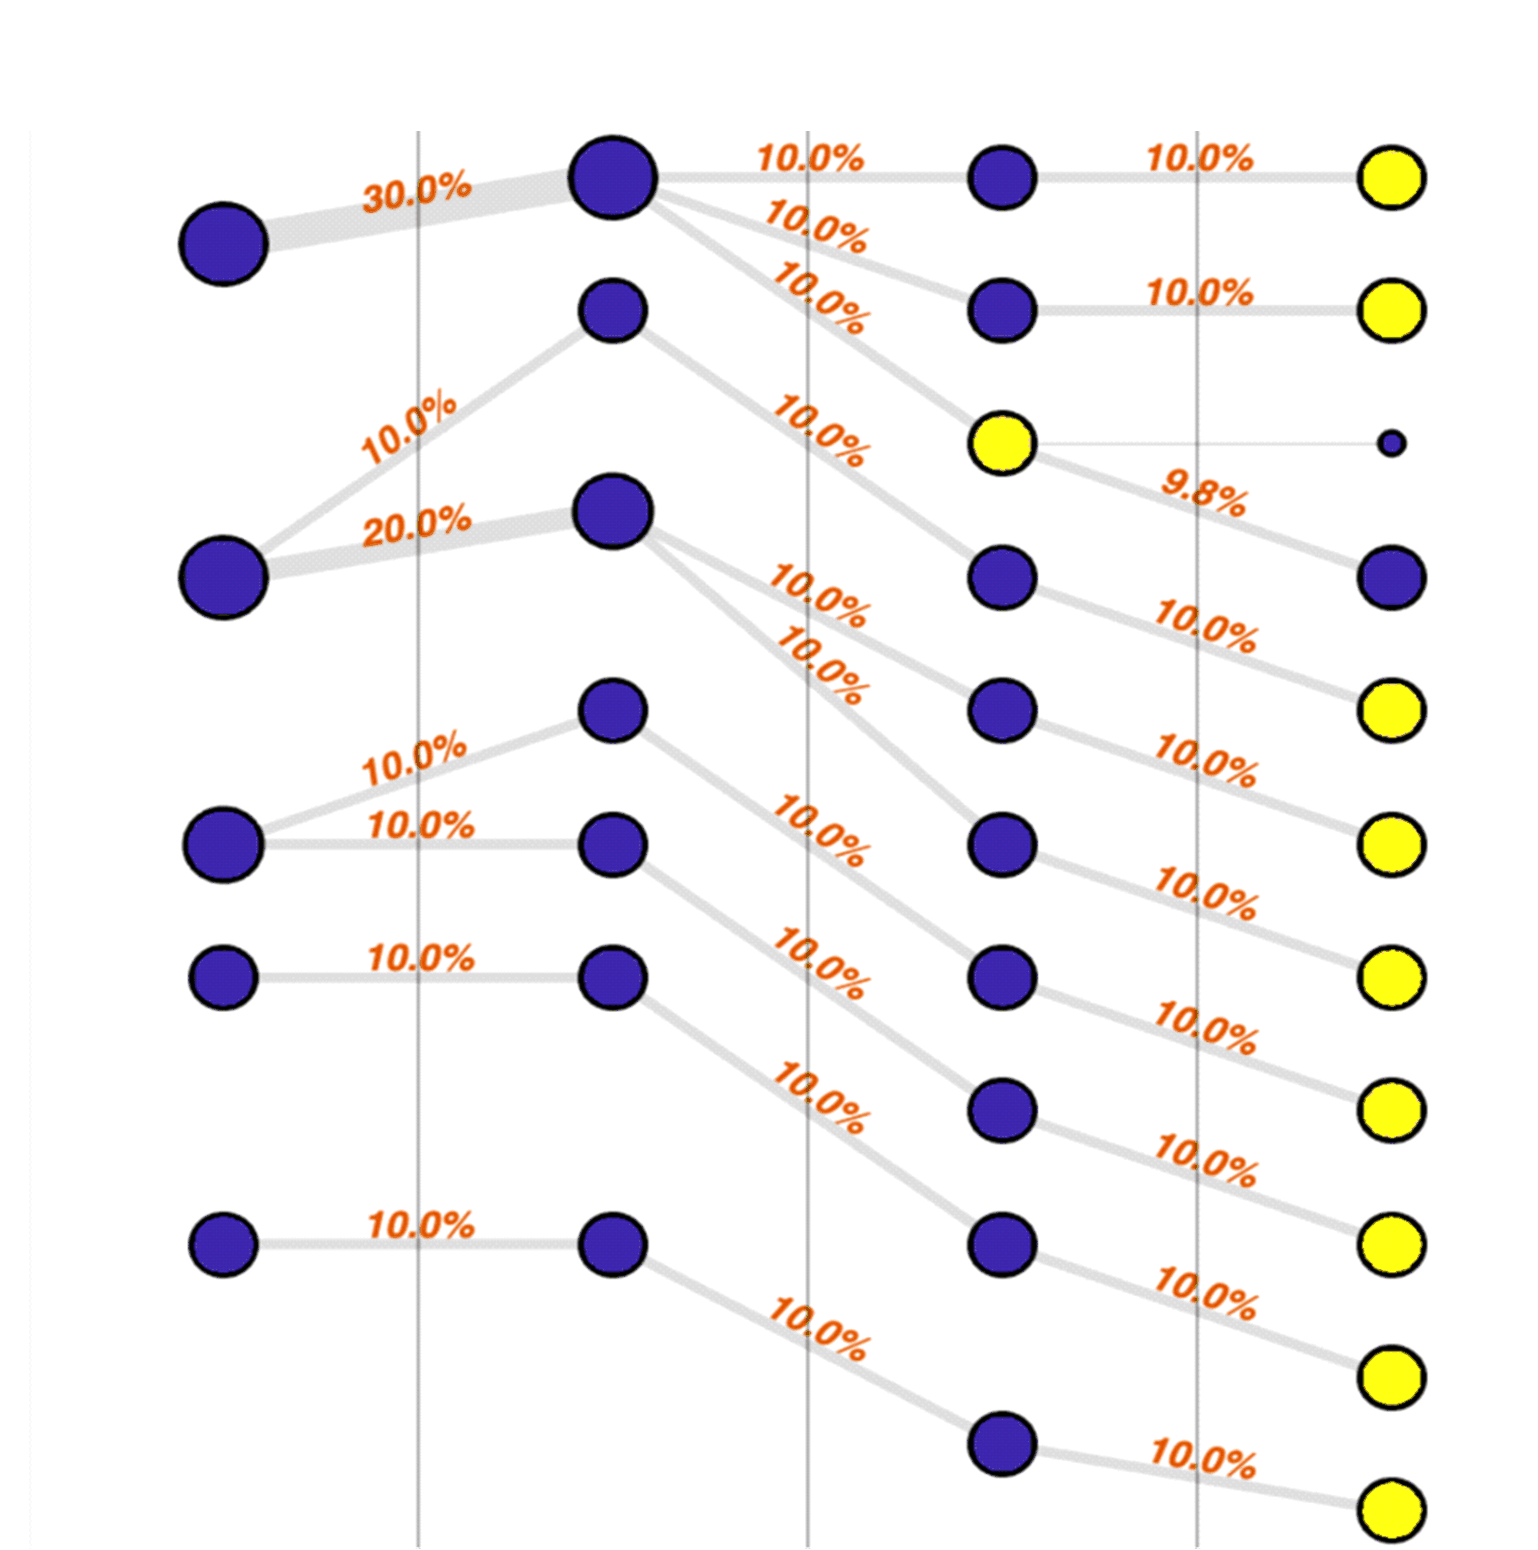
\includegraphics[width=0.2\linewidth]{assets/1004_gramixc/2.1.png}
  }
  \subcaptionbox{Cfg. attention map\label{fig:cifar10_GraMixC_attention}}{
    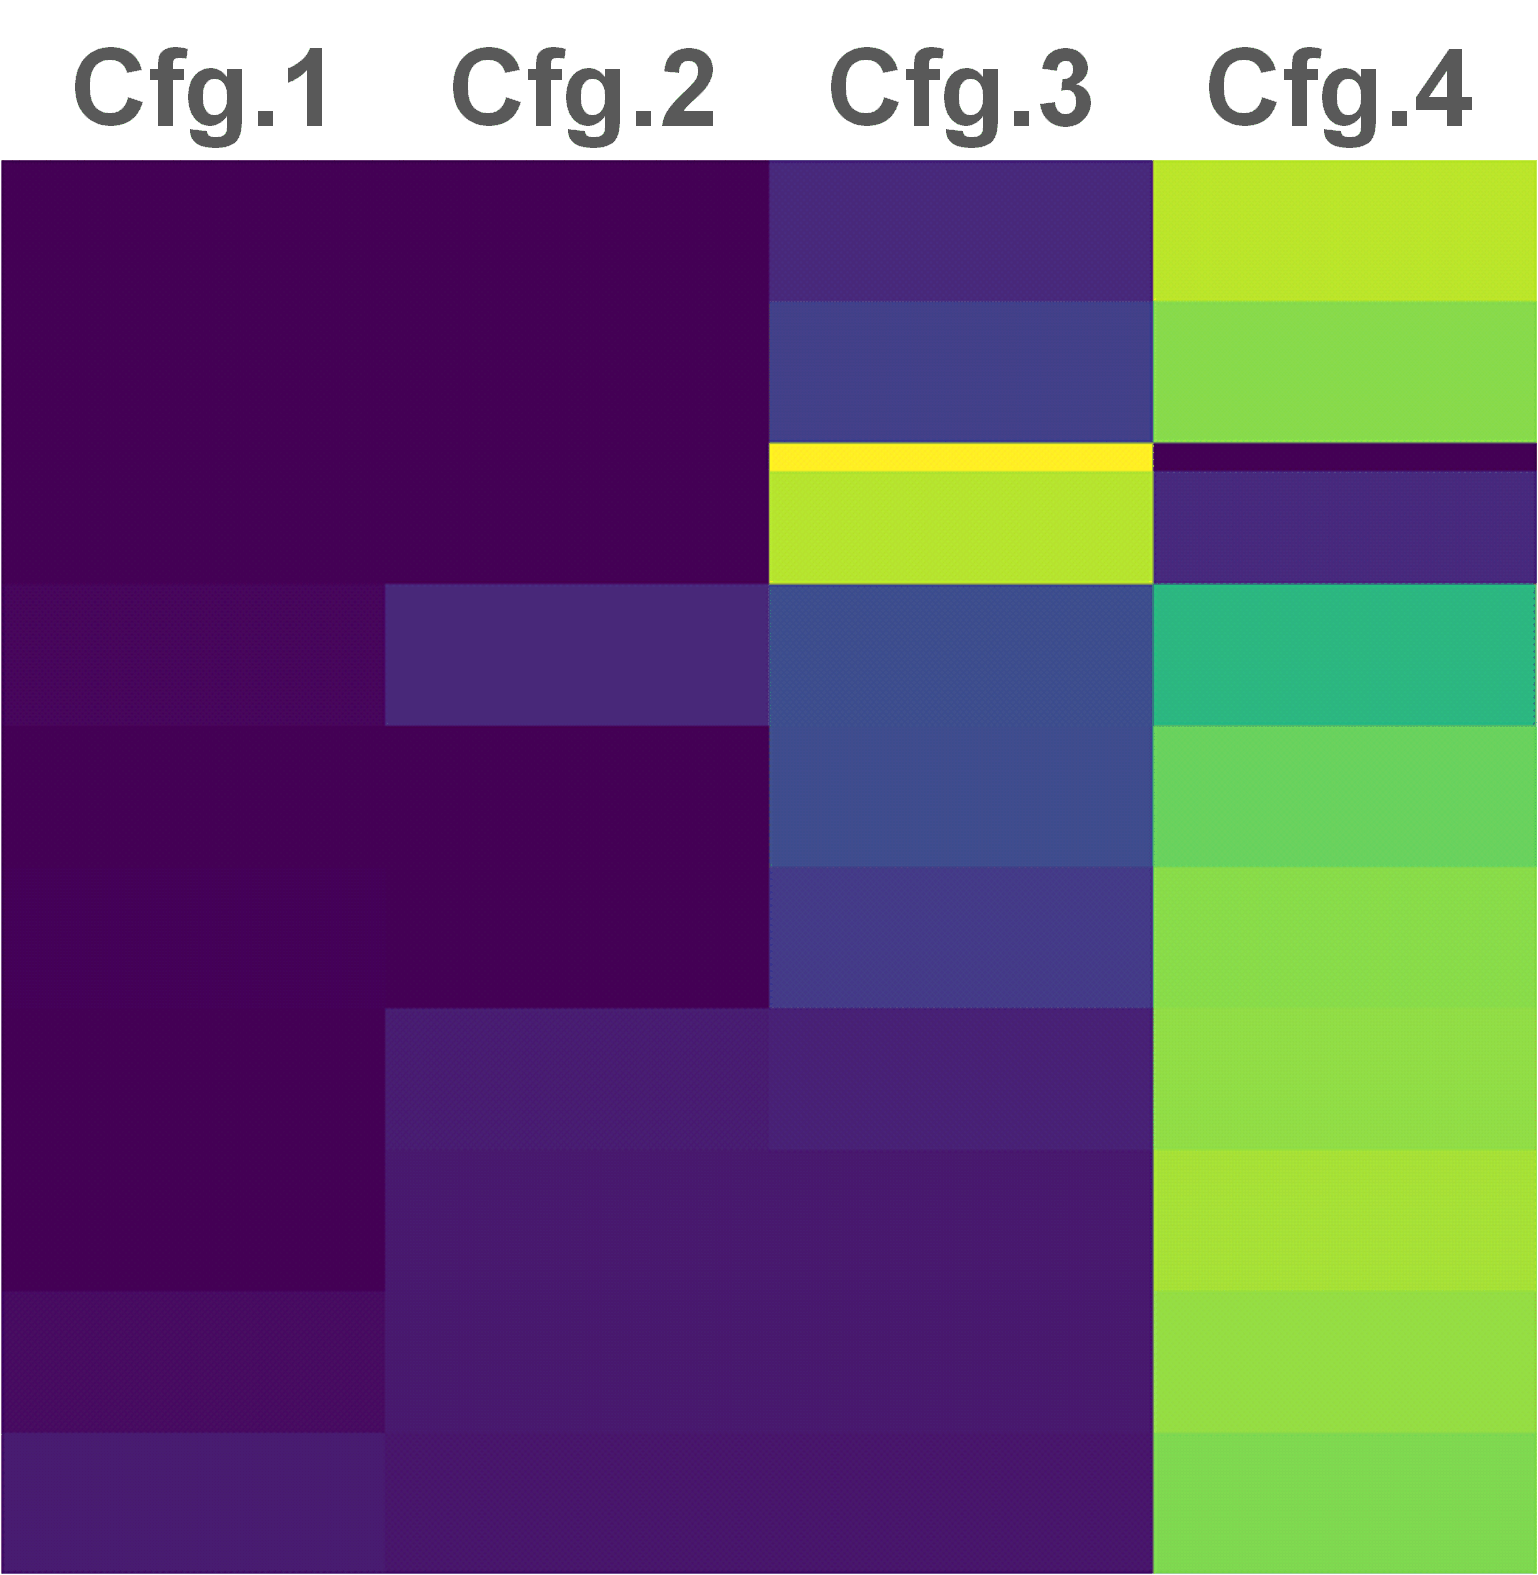
\includegraphics[width=0.2\linewidth]{assets/1004_gramixc/2.2.png}
  }
  \subcaptionbox{Reg. attention map\label{fig:cifar10_dino+reg_attentionl}}{
    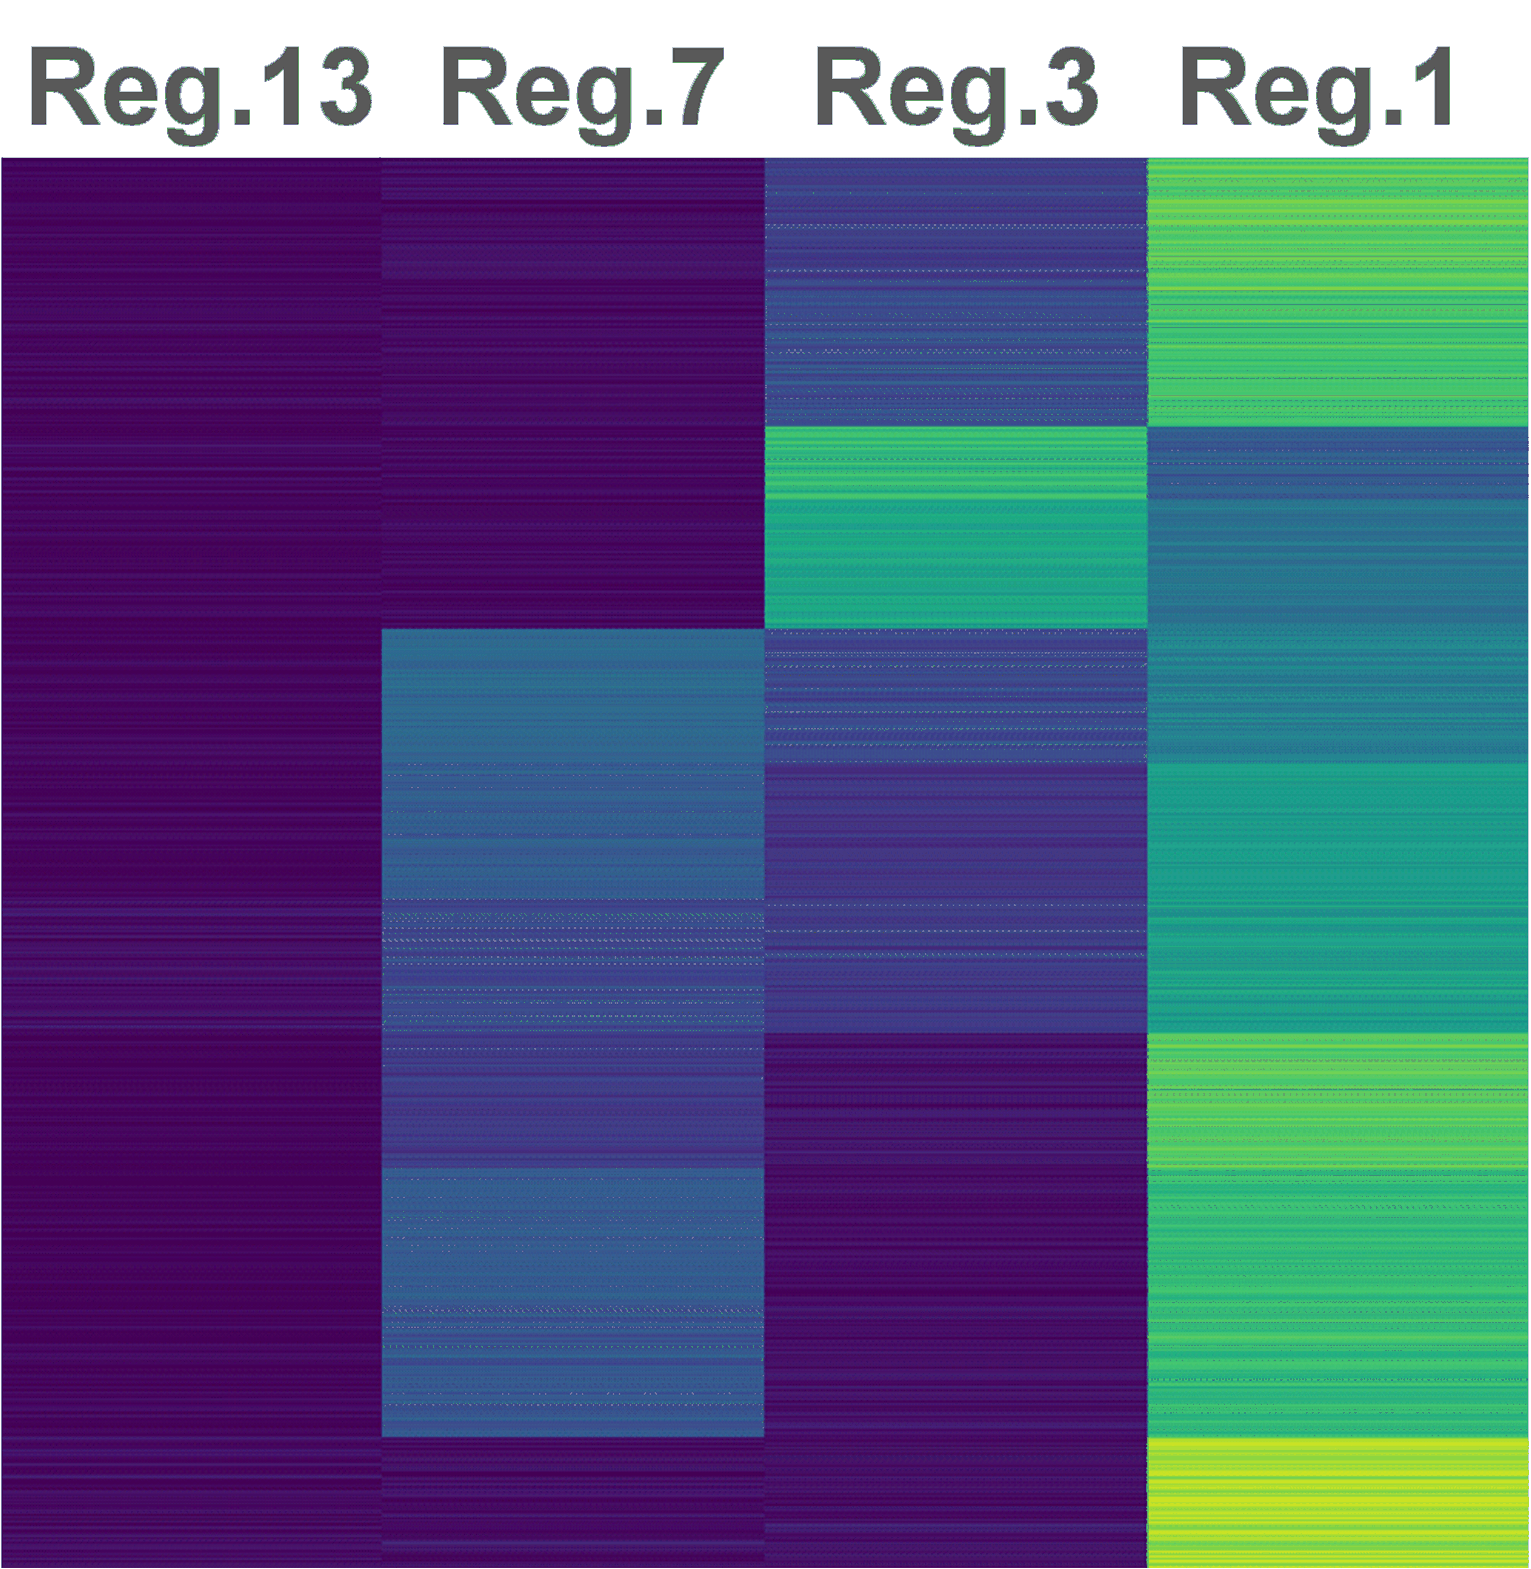
\includegraphics[width=0.2\linewidth]{assets/1004_gramixc/2.3.png}
  }
  \subcaptionbox{Reg. attention imgs\label{fig:cifar10_dino+reg_attentionl_map}}{
    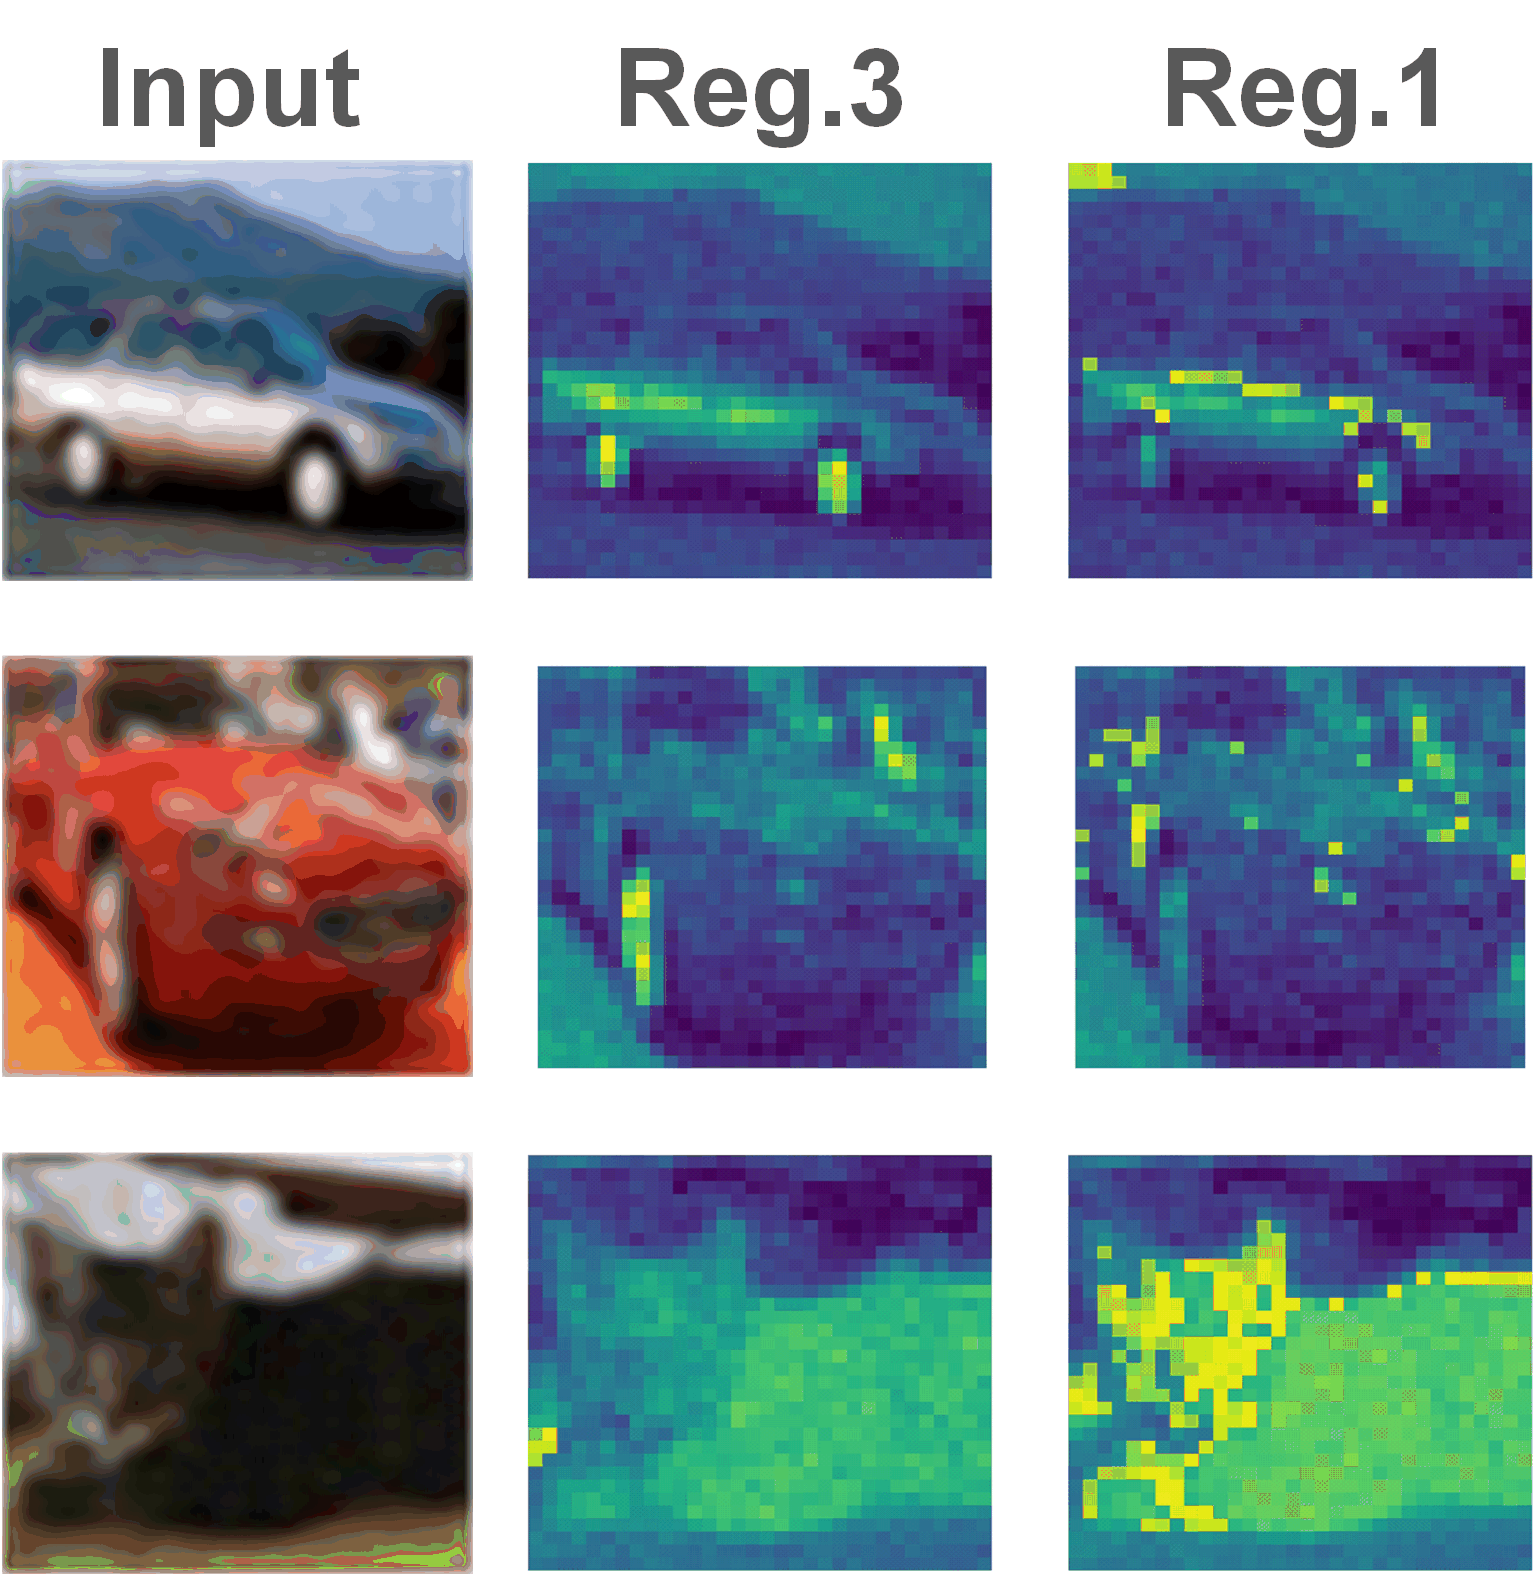
\includegraphics[width=0.2\linewidth]{assets/1004_gramixc/2.4.png}
  }
  \caption{
    Comparison of attention maps obtained from configurations and registers, rows for samples.
    \textbf{(a)}: Lineage diagram for configurations, near GT balls are marked yellow.
    \textbf{(b)}: Attention map of configuration tokens in an attention-based linear probing.
    \textbf{(c)}: Attention map of DINOv2-reg register tokens, mean of all patch norms is used.
    \textbf{(d)}: Attention maps over the register tokens, as images.
  }
  \label{fig:similar_behavior}
\end{figure}

\textbf{Key Results:}
\begin{itemize}[leftmargin=1.2em, itemsep=0.1em]
  \item Regression (DSNI): 3LP+GC improves over the 3LP baseline; 3LP+GMC further raises R$^2$ (up to $>0.9$), see Fig.~\ref{fig:dsmz_regression}.
  \item Ablation: Incrementally mixing configurations (GMC) consistently outperforms static train/test pairing (GC), Fig.~\ref{fig:dsmz_ablation}.
  \item Interpretability: Attention maps and lineage diagrams indicate configurations capture semantically meaningful structure (Fig.~\ref{fig:similar_behavior}).
  \item Design: GraMixC fuses configuration features with task predictors without modifying the backbone.
\end{itemize}


\textbf{Impact:} 
This work contributes to the growing field of self-supervised and unsupervised representation learning, with potential applications in materials science, molecular design, and any domain with configurable systems. Part of signature work research at Duke Kunshan University under Prof. Shixin Xu, focusing on unsupervised/semi-supervised methods for biomedical tasks.

\begin{figure}[ht]
  \centering
  \subcaptionbox{DSNI regression (3LP baseline vs. GC/GMC)\label{fig:dsmz_regression}}{
    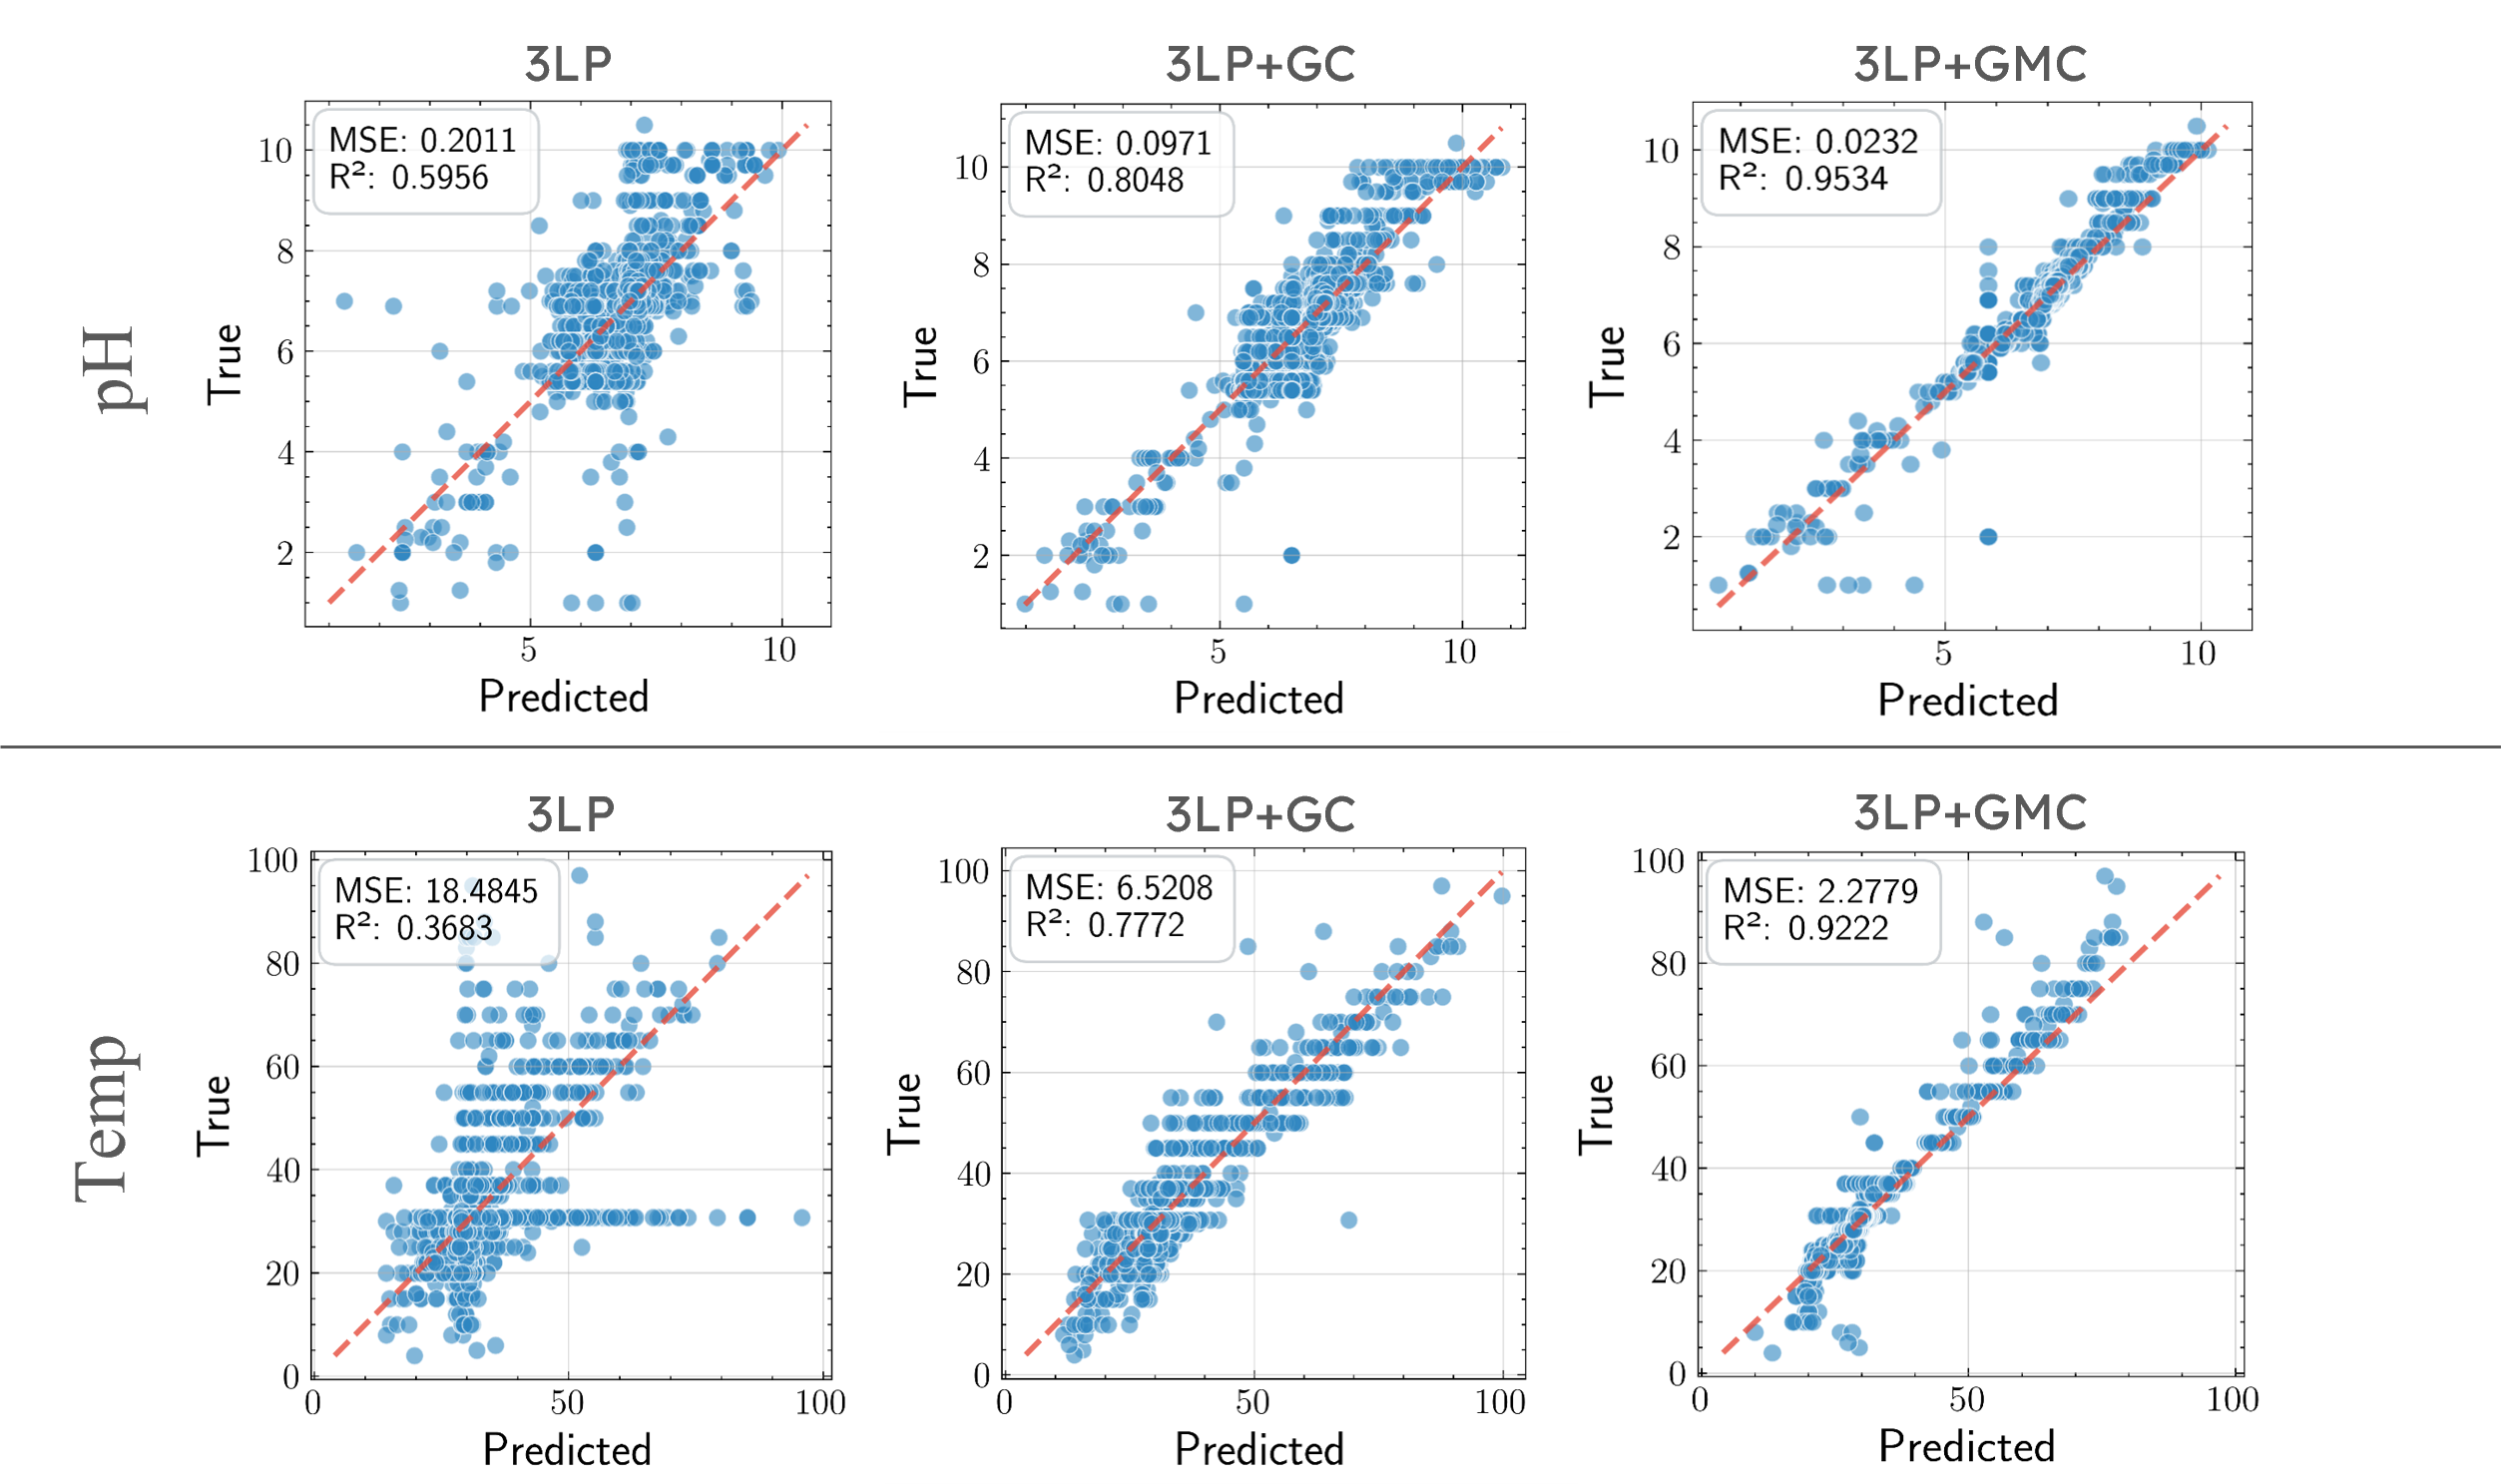
\includegraphics[width=0.48\linewidth]{assets/1004_gramixc/dsni_regression.png}
  }\hfill
  \subcaptionbox{DSNI ablation (mixing configurations)\label{fig:dsmz_ablation}}{
    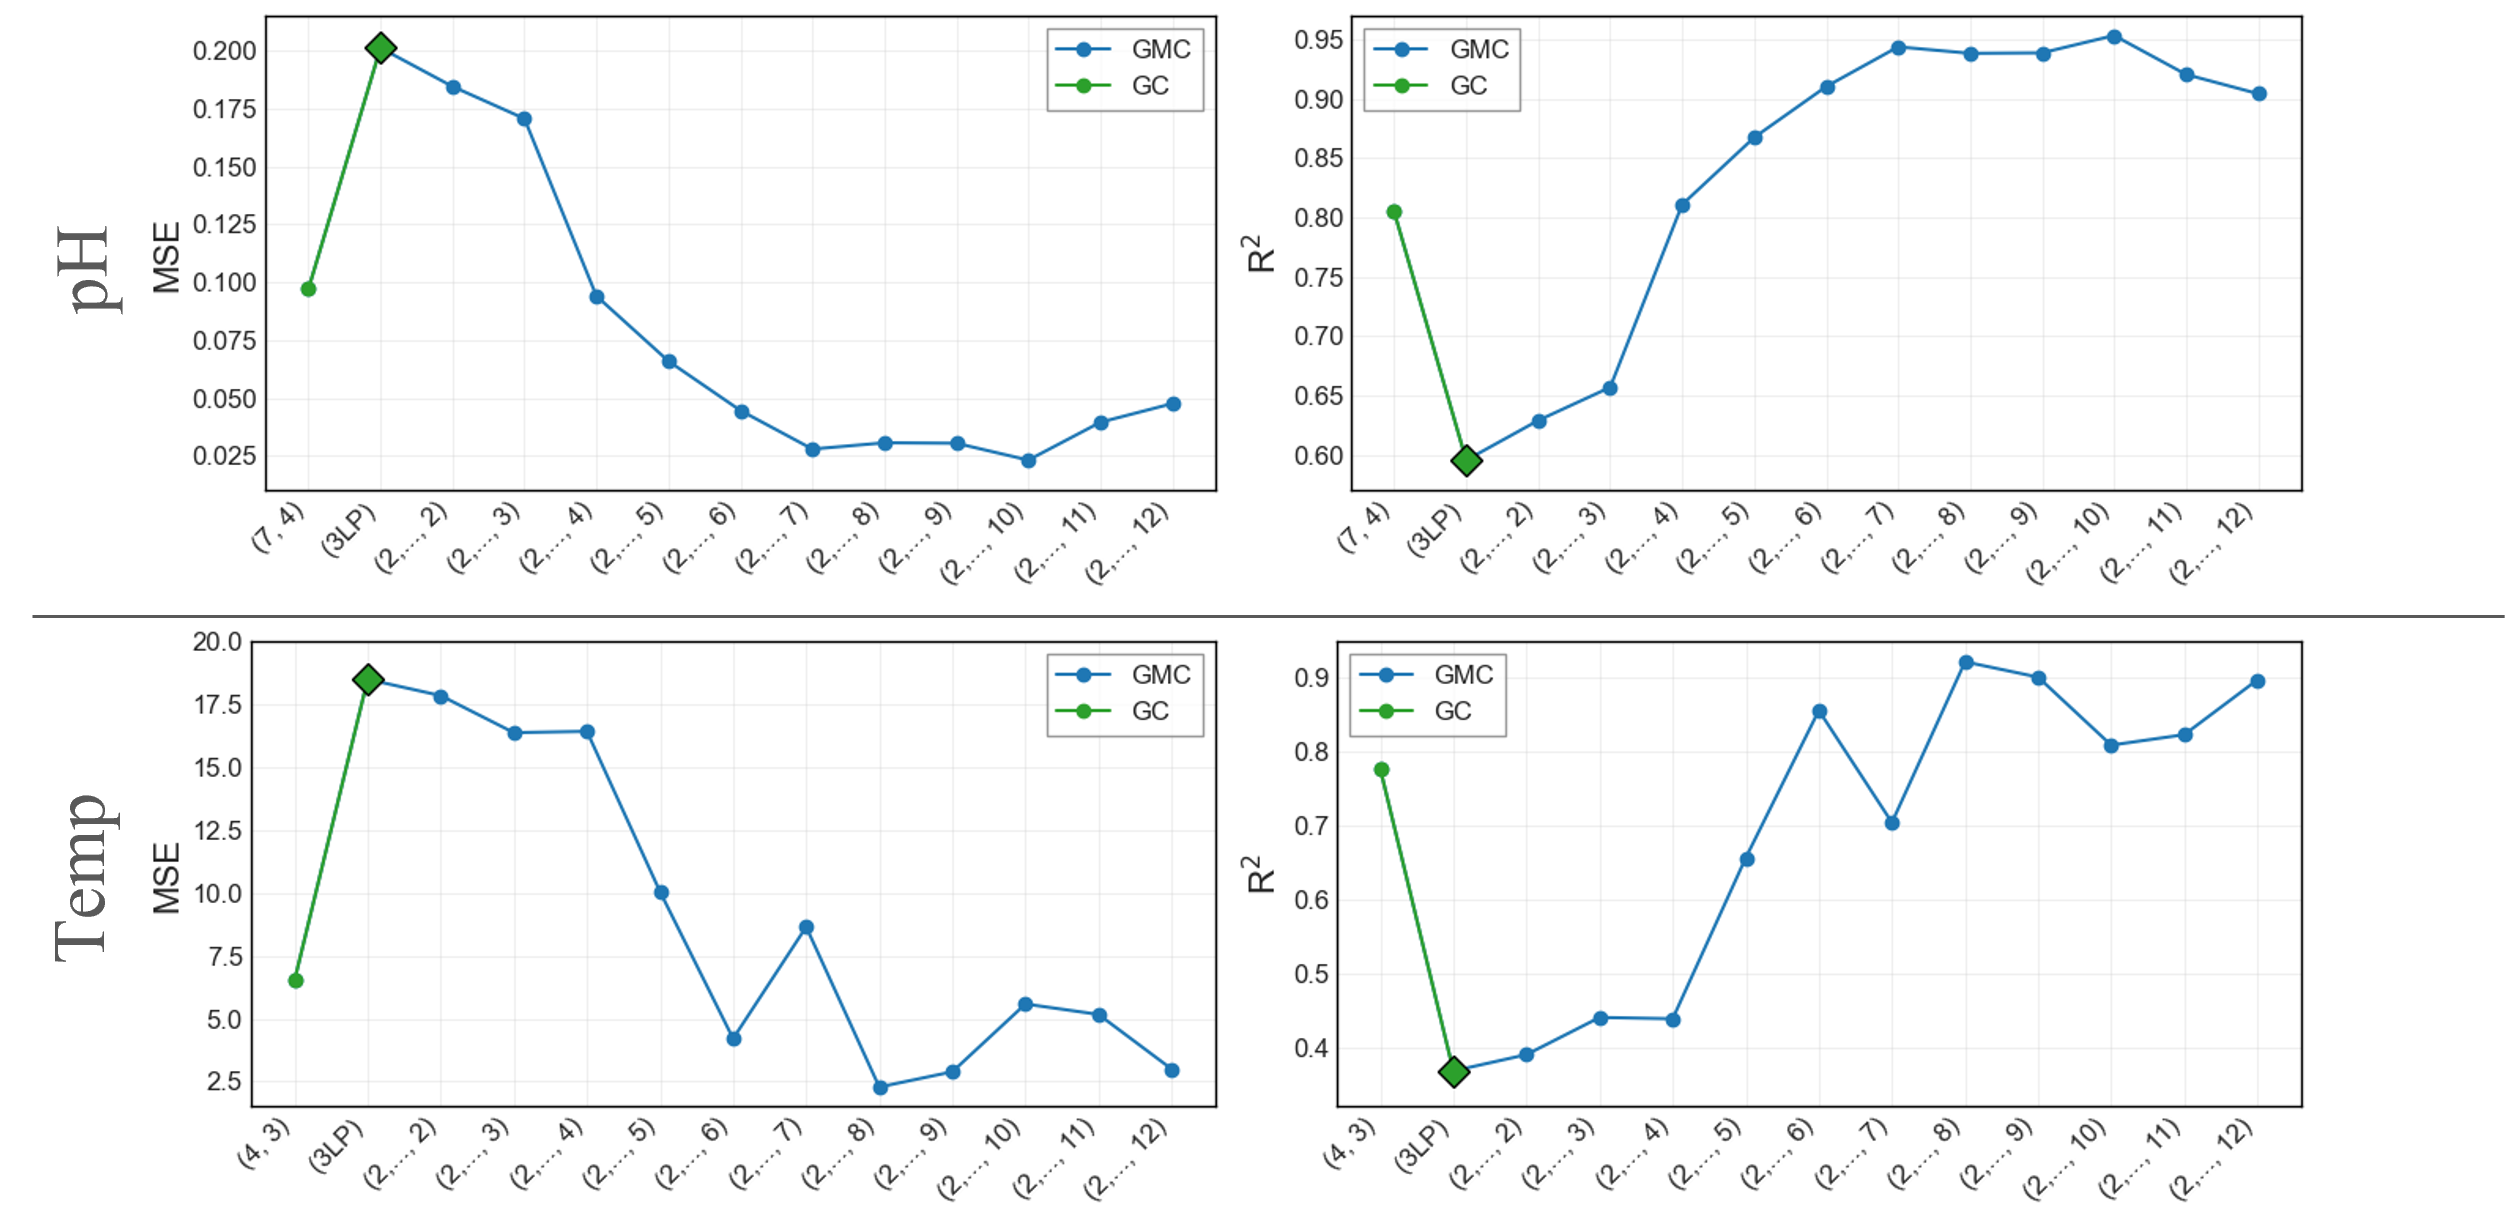
\includegraphics[width=0.48\linewidth]{assets/1004_gramixc/dsni_ablation.png}
  }
  \caption{Quantitative results on DSNI. (Left) Predicted vs. actual pH/temperature: 3LP+GC improves over 3LP; 3LP+GMC further increases R$^2$ (up to $>0.9$). (Right) Ablation: Incremental mixing (GMC) outperforms static train/test pairing (GC).}
\end{figure}

% ---------------------------------------------------------------------------
% PROJECT 3: InfantConfig
% ---------------------------------------------------------------------------

\addcontentsline{toc}{subsection}{Brain-Inspired Perspective on Configurations (BICS 2025)}
\ProjectEntry
{Brain-Inspired Perspective on Configurations: Unsupervised Similarity and Early Cognition}
{First Author}
{Theory, Unsupervised Learning, Brain-Inspired Computation}
{
  \bitem{Studies configurations from a cognitive perspective, relating unsupervised similarity and early cognition.}
  \bitem{Provides theoretical motivation for why configuration structure supports downstream prediction (complementary to GraMixC).}
  \bitem{Connects lineage diagrams, attention structure, and similarity to emergent representation geometry.}
}
{assets/1003_infantconfig/02a_schematic.png}
{\extlink{https://arxiv.org/abs/2510.19229}{arXiv preprint}}
{\badge{Brain-Inspired Computation} \badge{BICS 2025}}

\textbf{Technical Highlights:}
This work formalizes configurations as organizing structures that emerge from unsupervised similarity, offering a brain-inspired account of early category formation. We analyze how a lineage parameter \(\gamma\) controls hierarchical granularity and how energy components (attraction \(h_a\), repulsion \(h_r\)) shape stable configuration landscapes that support downstream learning.

\begin{figure}[ht]
  \centering
  \vspace{-0.5em}
  \subcaptionbox{Lineage (schem.)\label{fig:lineage_schem}}[0.25\linewidth]{%
    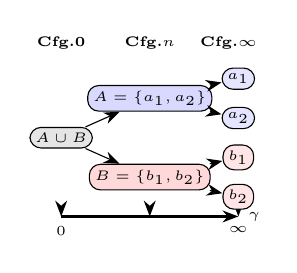
\begin{tikzpicture}[
    scale=0.5,
    node distance=8mm and 14mm,
    every node/.style={
        font=\tiny, 
        % minimum width=12mm, minimum height=5mm
    },
    level/.style={rectangle, rounded corners, draw=black, inner sep=2pt},
    ->,>={Stealth[length=2mm]}
]
    \draw[thick,->] (0.5,0) -- (5,0) node[right, font=\tiny] {$\gamma$};
    \draw[thick] (0.5,0.2) -- (0.5,0);
    \draw[thick] (2.75,0.2) -- (2.75,0);
    \draw[thick] (5,0.2) -- (5,0);
    \node[font=\tiny, below] at (0.5,0) {0};
    \node[font=\tiny, below] at (5,0) {$\infty$};
    \node[font=\tiny\bfseries, above] at (0.5,4) {Cfg.0};
    \node[font=\tiny\bfseries, above] at (2.75,4) {Cfg.$n$};
    \node[font=\tiny\bfseries, above] at (4.75,4) {Cfg.$\infty$};
    \node[level, fill=gray!20] (AB) at (0.5,2) {$A \cup B$};
    \node[level, fill=blue!15] (A) at (2.75,3) {$A=\{a_1,a_2\}$};
    \node[level, fill=red!15] (B) at (2.75,1) {$B=\{b_1,b_2\}$};
    \node[level, fill=blue!10] (A1) at (5,3.5) {$a_1$};
    \node[level, fill=blue!10] (A2) at (5,2.5) {$a_2$};
    \node[level, fill=red!10] (B1) at (5,1.5) {$b_1$};
    \node[level, fill=red!10] (B2) at (5,0.5) {$b_2$};
    \draw (AB) -- (A);
    \draw (AB) -- (B);
    \draw (A) -- (A1);
    \draw (A) -- (A2);
    \draw (B) -- (B1);
    \draw (B) -- (B2);
\end{tikzpicture}
%%
  }
  \subcaptionbox{Lineage (CIFAR)\label{fig:lineage_cifar}}[0.2\linewidth]{%
    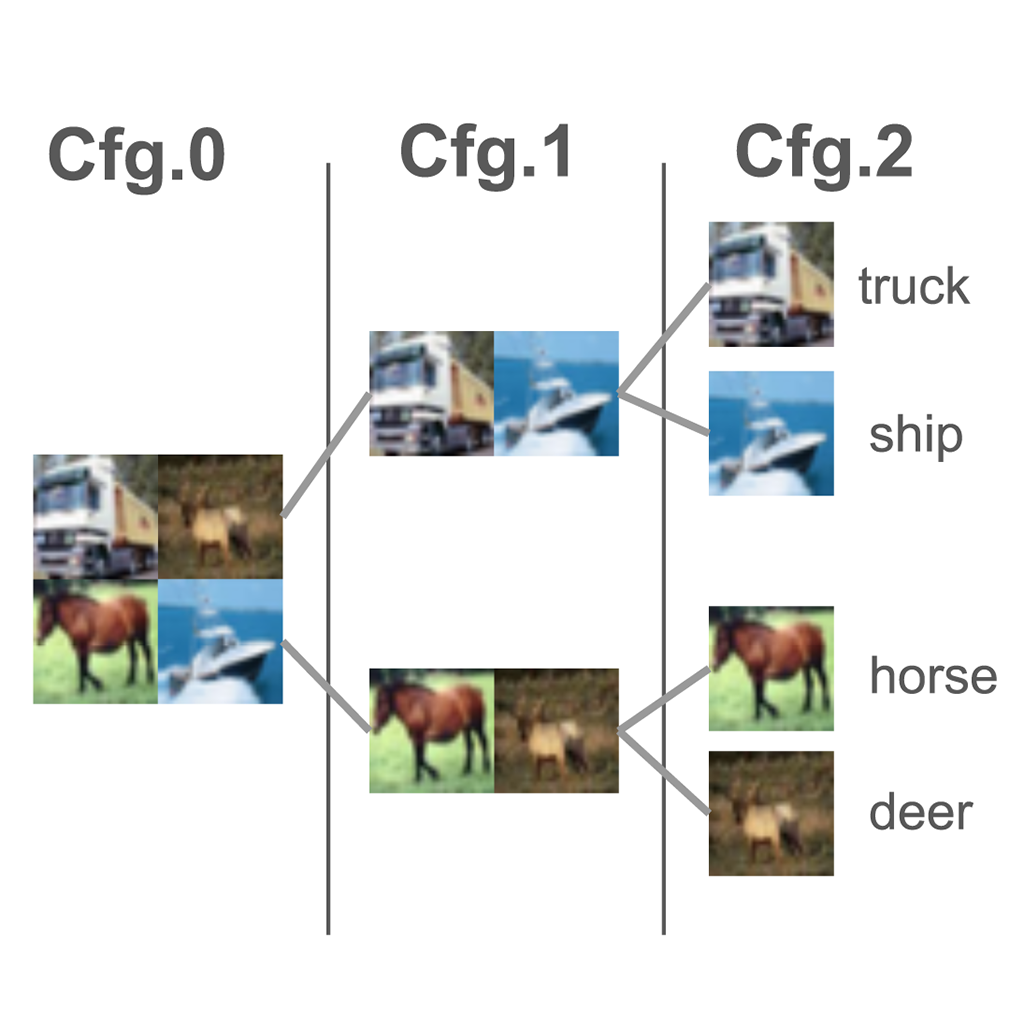
\includegraphics[width=\linewidth]{assets/1003_infantconfig/01_cifar10subset.png}%
  }
  \subcaptionbox{Energy (MNIST)\label{fig:energy_mnist}}[0.237\linewidth]{%
    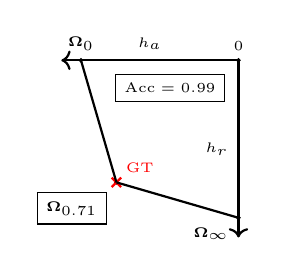
\begin{tikzpicture}[
    scale=0.5,
    every node/.style={
        font=\tiny,
    },
]
    \draw[->,thick] (0,0) -- (-4.5,0) node[midway, above] {$h_a$};
    \draw[->,thick] (0,0) -- (0,-4.5) node[midway, left] {$h_r$};
    \filldraw[black] (0,0) circle (1.2pt);
    \node[anchor=south] at (0,0) {0};
    \filldraw[black] (-4,0) circle (1.2pt);
    \node[anchor=south] at (-4,0) {$\mOmega_{0}$};
    \filldraw[black] (0,-4) circle (1.2pt);
    \node[anchor=north east] at (0,-4) {$\mOmega_{\infty}$};
    \filldraw[black] (-3.1,-3.1) circle (1.2pt);
    \node[anchor=north east] at (-3.1,-3.1) {$\boxed{\mOmega_{0.71}}$};
    \draw[red, thick] (-3.1-0.12, -3.1-0.12) -- (-3.1+0.12, -3.1+0.12);
    \draw[red, thick] (-3.1-0.12, -3.1+0.12) -- (-3.1+0.12, -3.1-0.12);
    \node[anchor=south west] at (-3.1, -3.1) {\color{red}GT};
    \draw[thick] (-4,0) -- (-3.1,-3.1);
    \draw[thick] (-3.1,-3.1) -- (0,-4);
    \node[anchor=north east] at (-0.1, -0.1) {
        $\boxed{\text{Acc}=0.99}$
};
\end{tikzpicture}%
  }
  \subcaptionbox{Energy (WHU)\label{fig:energy_whu}}[0.237\linewidth]{%
    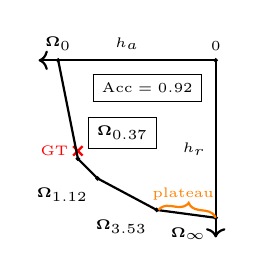
\begin{tikzpicture}[
    scale=0.5,
    every node/.style={
        font=\tiny,
    },
]
    \draw[->,thick] (0,0) -- (-4.5,0) node[midway, above] {$h_a$};
    \draw[->,thick] (0,0) -- (0,-4.5) node[midway, left] {$h_r$};
    \filldraw[black] (0,0) circle (1.2pt);
    \node[anchor=south] at (0,0) {0};
    \filldraw[black] (-4,0) circle (1.2pt);
    \node[anchor=south] at (-4,0) {$\mOmega_{0}$};
    \filldraw[black] (0,-4) circle (1.2pt);
    \node[anchor=north east] at (0,-4) {$\mOmega_{\infty}$};
    \filldraw[black] (-3.5,-2.5) circle (1.2pt);
    \node[anchor=south west] at (-3.5,-2.5) {$\boxed{\mOmega_{0.37}}$};
    \filldraw[black] (-3,-3) circle (1.2pt);
    \node[anchor=north east] at (-3,-3) {$\mOmega_{1.12}$};
    \filldraw[black] (-1.5,-3.8) circle (1.2pt);
    \node[anchor=north east] at (-1.5,-3.8) {$\mOmega_{3.53}$};
    \draw[red, thick] (-3.5-0.12, -2.3-0.12) -- (-3.5+0.12, -2.3+0.12);
    \draw[red, thick] (-3.5-0.12, -2.3+0.12) -- (-3.5+0.12, -2.3-0.12);
    \node[anchor=east] at (-3.5, -2.3) {\color{red}GT};
    \draw[thick] (-4,0) -- (-3.5,-2.5);
    \draw[thick] (-3.5,-2.5) -- (-3,-3);
    \draw[thick] (-3,-3) -- (-1.5,-3.8);
    \draw[thick] (-1.5,-3.8) -- (0,-4);
    \draw[orange,thick, decorate, decoration={brace, amplitude=4pt}]
    ($(-1.45,-3.8)$) -- ($(0,-4)$)
    node[midway, xshift=-0.5mm, yshift=2.5mm]{plateau};
    \node[anchor=north east] at (-0.1, -0.1) {
        $\boxed{\text{Acc}=0.92}$
};
\end{tikzpicture}%
  }
  \caption{
    Configuration lineage and energy landscapes. 
    \textbf{(a)\&(b)} Configuration lineages: $\gamma$ controls hierarchical granularity from coarse to fine. 
    \textbf{(c)\&(d)} Energy landscapes: Axes show attraction $h_a$ and repulsion $h_r$.}
  \label{fig:01_lineage_har}
\end{figure}

\textbf{Key Results:}
\begin{itemize}[leftmargin=1.2em, itemsep=0.1em]
  \item Hierarchical selectivity: superordinate categories stabilize at low \(\gamma\), basic-level categories at higher \(\gamma\), reflecting scale-dependent organization (Fig.~\ref{fig:04_a}).
  \item Novelty detection: energy distributions separate familiar vs. novel inputs (AUC \(\approx\) 0.87), echoing infant habituation paradigms (Fig.~\ref{fig:04_b}).
  \item Dynamic evolution: configurations achieve consistently lower 1/ARI than baselines during category evolution, indicating more stable organization (Fig.~\ref{fig:04_c}).
  \item Geometry: lineage diagrams and energy contours reveal interpretable structure that aligns with emergent representation geometry (Fig.~\ref{fig:01_lineage_har}).
\end{itemize}

\begin{figure}[ht]
  \centering
  \subcaptionbox{Hierarchical Selectivity\label{fig:04_a}}[0.33\linewidth]{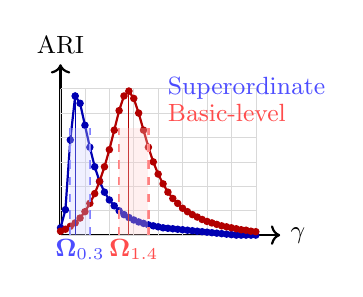
\begin{tikzpicture}[scale=0.62]
    \draw[->, thick] (0,0) -- (4.5,0) node[right, font=\small] {$\gamma$};
    \draw[->, thick] (0,0) -- (0,3.5) node[above, font=\small] {ARI};
    \draw[step=0.5, gray!30, very thin] (0,0) grid (4,3);
    \draw[thick, blue!70!black] plot[mark=*, mark size=1.5pt, mark options={fill=blue!70!black}] coordinates {
      (0.0, 0.15) (0.1, 0.52) (0.2, 1.95) (0.3, 2.85) (0.4, 2.70) (0.5, 2.25) (0.6, 1.80) (0.7, 1.40) (0.8, 1.10) (0.9, 0.88) (1.0, 0.72) (1.1, 0.60) (1.2, 0.50) (1.3, 0.42) (1.4, 0.36) (1.5, 0.31) (1.6, 0.27) (1.7, 0.24) (1.8, 0.21) (1.9, 0.19) (2.0, 0.17) (2.1, 0.15) (2.2, 0.14) (2.3, 0.13) (2.4, 0.12) (2.5, 0.11) (2.6, 0.10) (2.7, 0.09) (2.8, 0.08) (2.9, 0.07) (3.0, 0.06) (3.1, 0.05) (3.2, 0.04) (3.3, 0.03) (3.4, 0.02) (3.5, 0.01) (3.6, 0.00) (3.7, 0.00) (3.8, 0.00) (3.9, 0.00) (4.0, 0.00)
    };
    \draw[thick, red!70!black] plot[mark=*, mark size=1.5pt, mark options={fill=red!70!black}] coordinates {
      (0.0, 0.08) (0.1, 0.12) (0.2, 0.18) (0.3, 0.25) (0.4, 0.35) (0.5, 0.48) (0.6, 0.65) (0.7, 0.85) (0.8, 1.10) (0.9, 1.40) (1.0, 1.75) (1.1, 2.15) (1.2, 2.55) (1.3, 2.85) (1.4, 2.95) (1.5, 2.80) (1.6, 2.50) (1.7, 2.15) (1.8, 1.80) (1.9, 1.50) (2.0, 1.25) (2.1, 1.05) (2.2, 0.88) (2.3, 0.75) (2.4, 0.65) (2.5, 0.55) (2.6, 0.48) (2.7, 0.42) (2.8, 0.37) (2.9, 0.32) (3.0, 0.28) (3.1, 0.25) (3.2, 0.22) (3.3, 0.19) (3.4, 0.17) (3.5, 0.15) (3.6, 0.13) (3.7, 0.11) (3.8, 0.10) (3.9, 0.08) (4.0, 0.07) 
    };
    \draw[blue!70!black] (0.3, 0) -- (0.3, 2.85);
    \fill[blue!70!black] (0.3, 2.85) circle (2pt);
    \draw[red!70!black] (1.4, 0) -- (1.4, 2.95);
    \fill[red!70!black] (1.4, 2.95) circle (2pt);
    \draw[blue!50, dashed, thick] (0.2, 0) -- (0.2, 2.2);
    \draw[blue!50, dashed, thick] (0.6, 0) -- (0.6, 2.2);
    \fill[blue!20, opacity=0.3] (0.2, 0) rectangle (0.6, 2.2);
    \draw[red!50, dashed, thick] (1.2, 0) -- (1.2, 2.2);
    \draw[red!50, dashed, thick] (1.8, 0) -- (1.8, 2.2);
    \fill[red!20, opacity=0.3] (1.2, 0) rectangle (1.8, 2.2);
    \node[blue!70, font=\small, anchor=west] at (2, 3) {Superordinate};
    \node[red!70, font=\small, anchor=west] at (2, 2.5) {Basic-level};
    \node[font=\small, blue!70] at (0.4, -0.3) {$\mOmega_{0.3}$};
    \node[font=\small, red!70] at (1.5, -0.3) {$\mOmega_{1.4}$};
\end{tikzpicture}
%}
  \subcaptionbox{Novelty Detection\label{fig:04_b}}[0.33\linewidth]{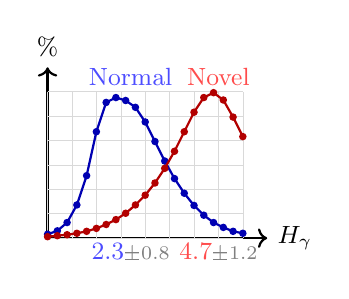
\begin{tikzpicture}[scale=0.62]
    \draw[->, thick] (0,0) -- (4.5,0) node[right, font=\small] {$H_\gamma$};
    \draw[->, thick] (0,0) -- (0,3.5) node[above, font=\small] {$\%$};
    \draw[step=0.5, gray!30, very thin] (0,0) grid (4,3);
    \draw[thick, blue!70!black] plot[mark=*, mark size=1.5pt, mark options={fill=blue!70!black}] coordinates {
      (0.0, 0.08) (0.2, 0.15) (0.4, 0.32) (0.6, 0.68) (0.8, 1.28) (1.0, 2.18) (1.2, 2.78) (1.4, 2.88) (1.6, 2.82) (1.8, 2.68) (2.0, 2.38) (2.2, 1.98) (2.4, 1.58) (2.6, 1.22) (2.8, 0.92) (3.0, 0.67) (3.2, 0.47) (3.4, 0.32) (3.6, 0.22) (3.8, 0.14) (4.0, 0.10)
    };
    \node[blue!70, font=\small] at (1.7, 3.3) {Normal};
    \node[blue!70, font=\small] at (1.7, -0.3) {2.3\s{0.8}};
    \draw[thick, red!70!black] plot[mark=*, mark size=1.5pt, mark options={fill=red!70!black}] coordinates {
      (0.0, 0.03) (0.2, 0.05) (0.4, 0.07) (0.6, 0.10) (0.8, 0.14) (1.0, 0.20) (1.2, 0.28) (1.4, 0.38) (1.6, 0.51) (1.8, 0.68) (2.0, 0.88) (2.2, 1.13) (2.4, 1.43) (2.6, 1.78) (2.8, 2.18) (3.0, 2.58) (3.2, 2.88) (3.4, 2.98) (3.6, 2.83) (3.8, 2.48) (4.0, 2.08)
    };
    \node[red!70, font=\small] at (3.5, 3.3) {Novel};
    \node[red!70, font=\small] at (3.5, -0.3) {4.7\s{1.2}};
\end{tikzpicture}
%}
  \hspace{-1em}
  \subcaptionbox{Dynamic Evolution\label{fig:04_c}}[0.33\linewidth]{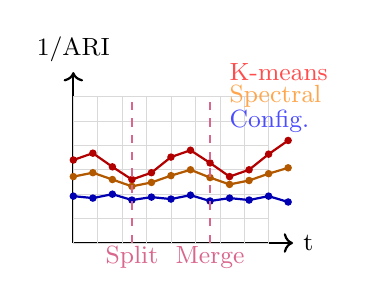
\begin{tikzpicture}[scale=0.62]
    \draw[->, thick] (0,0) -- (4.5,0) node[right, font=\small] {t};
    \draw[->, thick] (0,0) -- (0,3.5) node[above, font=\small] {1/ARI};
    \draw[step=0.5, gray!30, very thin] (0,0) grid (4,3);
    \draw[thick, red!70!black] plot[mark=*, mark size=1.5pt, mark options={fill=red!70!black}] coordinates {
      (0.0, 1.70) (0.4, 1.84) (0.8, 1.56) (1.2, 1.30) (1.6, 1.44) (2.0, 1.76) (2.4, 1.90) (2.8, 1.64) (3.2, 1.36) (3.6, 1.50) (4.0, 1.82) (4.4, 2.10)
    };
    \node[red!70, font=\small, anchor=west] at (3, 3.5) {K-means};
    \draw[thick, orange!70!black] plot[mark=*, mark size=1.5pt, mark options={fill=orange!70!black}] coordinates {
      (0.0, 1.36) (0.4, 1.44) (0.8, 1.30) (1.2, 1.16) (1.6, 1.24) (2.0, 1.38) (2.4, 1.50) (2.8, 1.34) (3.2, 1.20) (3.6, 1.28) (4.0, 1.42) (4.4, 1.54)
    };
    \node[orange!70, font=\small, anchor=west] at (3, 3) {Spectral};
    \draw[thick, blue!70!black] plot[mark=*, mark size=1.5pt, mark options={fill=blue!70!black}] coordinates {
      (0.0, 0.96) (0.4, 0.92) (0.8, 1.00) (1.2, 0.88) (1.6, 0.94) (2.0, 0.90) (2.4, 0.98) (2.8, 0.86) (3.2, 0.92) (3.6, 0.88) (4.0, 0.96) (4.4, 0.84)
    };
    \node[blue!70, font=\small, anchor=west] at (3, 2.5) {Config.};
    \draw[purple!60, dashed, thick] (1.2, 0) -- (1.2, 3);
    \draw[purple!60, dashed, thick] (2.8, 0) -- (2.8, 3);
    \node[purple!60, font=\small] at (1.2, -0.3) {Split};
    \node[purple!60, font=\small] at (2.8, -0.3) {Merge};
\end{tikzpicture}
%}
  \caption{
    Brain-inspired capabilities of configurations.
    \textbf{(a)} Superordinate categories emerge at low $\gamma$ (0.2--0.6), basic-level at high $\gamma$ (1.2--1.8). Plateaus show stable organizational scales.
    \textbf{(b)} Energy distributions distinguish novel from familiar stimuli (87\% AUC), paralleling infant habituation.
    \textbf{(c)} Configurations achieve stable 35\% lower 1/ARI than other two baselines during category evolution.
  }
  \label{fig:04}
\end{figure}

\textbf{Impact:}
By linking unsupervised similarity, hierarchical lineage, and energy-based organization, this project offers a principled, cognitively motivated view of how early concepts can form without labels. The framework complements GraMixC by explaining why configuration structure is predictive, and it suggests broader applications in domains where category structure and novelty signals emerge from unlabeled data.


% ---------------------------------------------------------------------------
% PROJECT 2: TamKwok
% ---------------------------------------------------------------------------
\addcontentsline{toc}{subsection}{EEG/EMG Vigilance Classification (PNAS Nexus under review, CNS 2025)}
\ProjectEntry
{EEG/EMG Vigilance Classification under Martian Photoperiod (T24.66)}
{First Student Author}
{EEG/EMG, FFT/Wavelet, Sleep \& Memory, Photoperiod}
{
  \bitem{Tested whether mammals adapt to Mars-like 12.33h light:12.33h dark cycles (T24.66).}
  \bitem{Found circadian realignment without free-running; ultradian noise increased under T24.66.}
  \bitem{Observed advanced siesta peak and increased midnight sleep; waking theta (8--12 Hz) attenuated at night.}
  \bitem{Night-time short-term object memory attenuated due to altered response to familiar objects; novelty response intact.}
}
{assets/1002_tamkwok/00_.png}
{\extlink{https://www.qqgjyx.com/files/p02-TamKwok-CNS2025.pdf}{CNS 2025 paper} \quad \extlink{https://qqgjyx.my.canva.site/s02-tamkwok-srs}{Slides}}
{\badge{CNN} \badge{PNAS Nexus under review} \badge{CNS 2025}}

\vspace{1em}

\textbf{Technical Highlights:}
We investigate mammalian adaptation to a Martian-length day (T24.66) using laboratory mice. The regime lengthens intrinsic period (\(\tau\)) enabling realignment to the slightly longer photoperiod without free running. Spectral analyses reveal preserved circadian power but amplified ultradian components; sleep architecture shifts and night-time waking theta decreases.

\begin{figure}[ht]
  \centering
  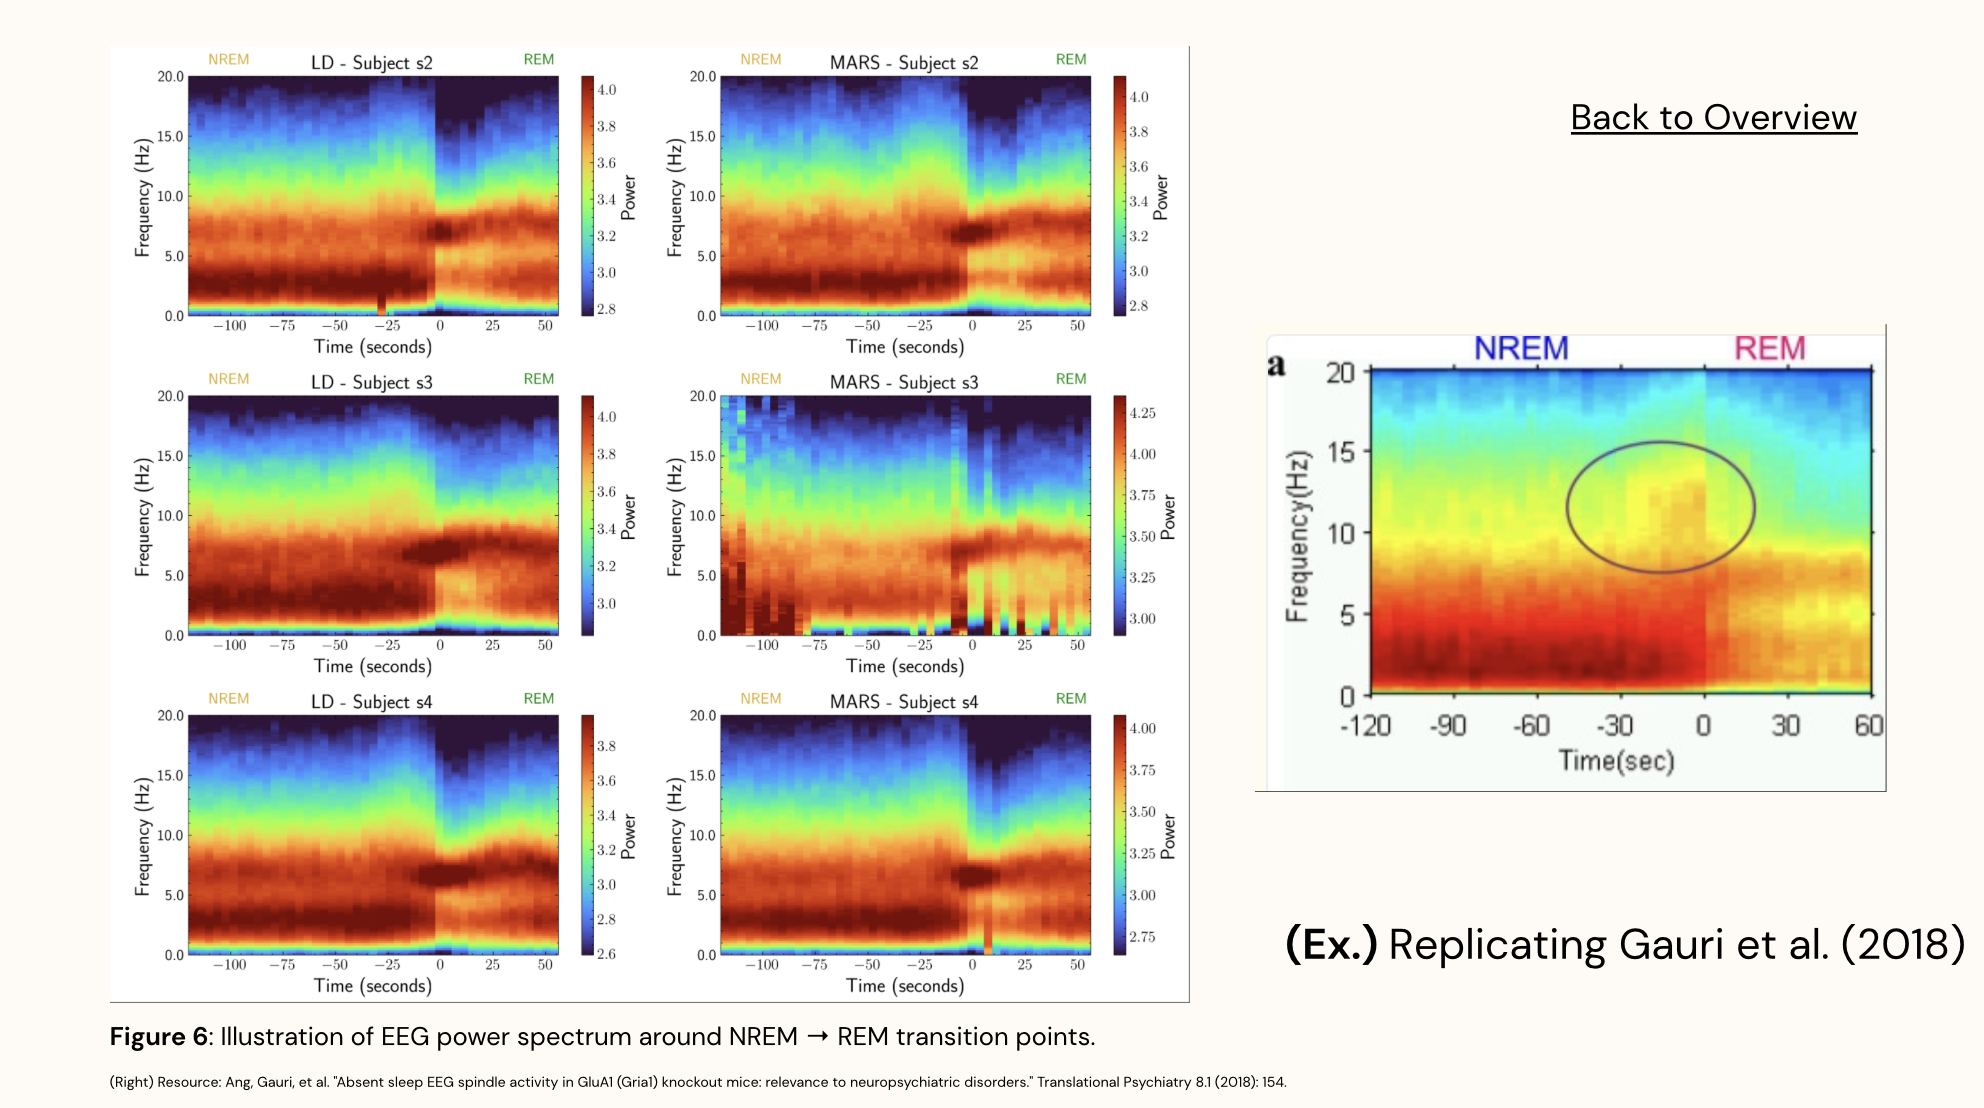
\includegraphics[width=0.85\linewidth]{assets/1002_tamkwok/01_.png}
  \caption{EEG spectral analyses around state transitions under T24.66. Wavelet/FFT-based spectra highlight attenuated waking theta (8--12 Hz) at night and altered sleep timing relative to T24.}
  \label{fig:t2466_spectra}
\end{figure}

\textbf{Methodology:}
\begin{itemize}[leftmargin=1.2em, itemsep=0.1em]
  \item Entrainment protocol: 12.33h light : 12.33h dark (T24.66) vs. T24 controls
  \item EEG/EMG recording; spectral analyses via fast Fourier transform (FFT) and wavelets
  \item Behavioral assessments: rest–activity rhythm, sleep timing, object memory assays
\end{itemize}

\textbf{Key Findings:}
\begin{itemize}[leftmargin=1.2em, itemsep=0.1em]
  \item Circadian: \(\tau\) lengthened; rhythms realigned with T24.66 without free running; circadian power not dampened
  \item Ultradian: Increased ultradian spectral power (FFT/wavelet)
  \item Sleep: Advanced siesta peak; increased midnight sleep; time-of-day dependent changes
  \item EEG: Night-time waking theta (8--12 Hz) attenuated
  \item Memory: Night-time short-term object memory attenuated due to altered response to familiar objects; novelty response spared
\end{itemize}

\textbf{Impact:} Findings suggest that adapting to a slightly non-24h photoperiod (T24.66) is feasible but entails neurophysiological trade-offs in sleep, alertness, and memory—relevant for space mission planning.

\vspace{1em}

\textbf{Publications:}
\begin{itemize}[leftmargin=1.2em, itemsep=0.1em]
  \item Shu Kit Eric Tam, Juntang Wang, Aleksandra Stryjska, Pascal Grange, Sze Chai Kwok. "Martian Photoperiod Attenuates Waking Theta Activity at Night and Disrupts Short-term Object Memory in Mice Despite Circadian Realignment." PNAS Nexus (under review).
  \item Shu Kit Eric Tam, Juntang Wang, Sze Chai Kwok. "Can the mammalian circadian system adapt to the Martian photoperiod?" Presented at CNS 2025.
\end{itemize}

% ---------------------------------------------------------------------------
% PROJECT 1: LK99
% ---------------------------------------------------------------------------

\addcontentsline{toc}{subsection}{Analyzing Temperature-Induced Phase Transitions in LK99 (MC17)}
\ProjectEntry
{Analyzing Temperature-Induced Phase Transitions in Pb$_{10-x}$Cu$_x$(PO$_4$)$_6$O}
{Research Independent Study with Prof. Xiawa Wang}
{Phonon/exciton dynamics}
{
  \bitem{Investigated LK-99 thermal behavior (300--500 K) via temperature-dependent XRD, Raman spectroscopy, and DSC.}
  \bitem{Observed reversible structural transitions in XRD (new/shifted peaks) correlating with resistivity jumps.}
  \bitem{Conducted density functional theory (DFT) analysis to interpret observed transitions and spectra.}
  \bitem{Raman modes shift in tandem with resistivity transition; DSC shows no pronounced latent heat.}
  \bitem{Results suggest either minor impurity (e.g., Cu$_2$S) contribution or subtle intrinsic lattice transformation.}
}
{assets/1001_lk99/00_.png}
{\extlink{https://online.flippingbook.com/view/299339187/111/}{MC17 paper} \quad \extlink{https://www.qqgjyx.com/files/p01-LK99-MC17.pdf}{Poster}}
{\badge{Materials Chemistry} \badge{DFT} \badge{MC17}}

\textbf{Technical Highlights:}
We examine temperature-sensitive structural responses in LK-99 that align with electrical resistivity changes. Reversible XRD peak evolution between 300--500 K and concomitant Raman shifts indicate a repeatable transition regime, while DSC lacks strong latent heat signatures.

\textbf{Methodology:}
\begin{itemize}[leftmargin=1.2em, itemsep=0.1em]
  \item Variable-temperature XRD to identify reversible phase/structure evolution
  \item Raman spectroscopy to track vibrational mode shifts across the transition
  \item Differential scanning calorimetry (DSC) to probe latent heat signatures
  \item Resistivity measurements correlated with structural/spectral changes
  \item Density functional theory (DFT) analysis to interpret observed transitions and spectra
\end{itemize}

\textbf{Key Findings:}
\begin{itemize}[leftmargin=1.2em, itemsep=0.1em]
  \item Reversible structural transition correlates with resistivity jumps (300--500 K)
  \item Raman modes shift coherently with structural/electrical changes
  \item Absence of strong DSC peak suggests subtle transformation or low-fraction impurity phase
  \item Thermal/electrical repeatability indicates potential for sensing/switching applications
\end{itemize}

\textbf{Impact:} 
The coupling between structure and electrical response highlights LK-99 as a temperature-sensitive material of interest for functional electronics. Disentangling impurity effects from intrinsic copper-doped lattice behavior requires further microstructural analysis.

% ---------------------------------------------------------------------------
% PROJECT 0: HSI
% ---------------------------------------------------------------------------

\addcontentsline{toc}{subsection}{Unsupervised Segmentation in Hyperspectral Imaging}
\ProjectEntry
{Unsupervised Segmentation in Hyperspectral Imaging}
{Summer Research \& Independent Study with Prof. Xiaobai Sun, Prof. Nikos Pitsianis, Dimitrios Floros}
{Python, SG-t-SNE-\textPi, Spectral Methods, Community Detection}
{
  \bitem{Studied precursor clustering and community detection methods, collecting over 5 methods and more than 10 datasets for hyperspectral imaging segmentation.}
  \bitem{Implemented and optimized SG-t-SNE-\textPi{} algorithm for dimensionality reduction preserving local and global structure.}
  \bitem{Utilized k-nearest neighbor graphs, Stochastic Graph t-SNE, and Parallel Clustering with Resolution Variation for unsupervised segmentation.}
  \bitem{Developed Python packages mheatmap and pysgtsnepi for HSI data processing, achieving 600+ GitHub stars community adoption.}
  \bitem{Worked with Python (scikit-learn), MATLAB, and Julia for implementation and validation.}
}
{assets/1000_hsi/00_.png}
{\extlink{https://www.qqgjyx.com/files/p00-HSI.pdf}{Poster}}
{\badge{HSI} \badge{Graph} \badge{Unsupervised Learning}}

\textbf{Technical Highlights:}
Hyperspectral images contain hundreds of spectral bands per pixel, creating extremely high-dimensional data that is challenging to segment without labels. This project leverages spectral graph theory to build a similarity graph where pixels are nodes and edges encode spectral similarity.

\textbf{Methodology:}
\begin{itemize}[leftmargin=1.2em, itemsep=0.1em]
  \item Construct k-nearest neighbor graph in spectral space using efficient approximate nearest neighbor search
  \item Apply SG-t-SNE-\textPi{} to embed the graph structure into 2D/3D space while preserving cluster structure
  \item Use community detection to identify coherent spectral regions corresponding to materials or land cover types
  \item Validate segmentations against ground truth using metrics like adjusted Rand index and normalized mutual information
\end{itemize}

\textbf{Key Findings:}
\begin{itemize}[leftmargin=1.2em, itemsep=0.1em]
  \item BlueRed consistently outperforms traditional baselines on HSI clustering
  \item Robust to spectral noise and spatial variability; produces coherent segments
\end{itemize}

\textbf{Impact:} 
The approach sets a stronger baseline for unsupervised HSI analysis with practical implications in agriculture, climate, remote sensing, and medical diagnostics. Future work: improve computational efficiency and extend to more HSI scenarios.


% ============================================================================
% SOFTWARE TOOLS (4–5 pages)
% ============================================================================
% ============================================================================
% SOFTWARE TOOLS
% ============================================================================

\section*{Software Tools \& Open Source Contributions}
\addcontentsline{toc}{section}{Software Tools \& Open Source}

% ---------------------------------------------------------------------------
% TOOL 2: mheatmap
% ---------------------------------------------------------------------------

\addcontentsline{toc}{subsection}{mheatmap: Proportional Heatmaps}
\ProjectEntry
{mheatmap: Proportional Heatmaps with Spectral Reordering}
{Creator \& Maintainer}
{Python, NumPy, Matplotlib, Spectral Graph Theory}
{
  \bitem{Developed Python package for creating proportional heatmaps where cell sizes reflect data magnitude.}
  \bitem{Implemented spectral reordering algorithms (Fiedler vector, spectral seriation) to reveal hidden structure.}
  \bitem{Achieved 600+ GitHub stars and widespread adoption in bioinformatics, systems biology, and network analysis.}
  \bitem{Package has been cited in peer-reviewed publications and used in production data analysis pipelines.}
  \bitem{Maintained comprehensive documentation with tutorials, examples, and API reference.}
}
{assets/2002_mheatmap/02b_mheatmap.png}
{\extlink{https://github.com/qqgjyx/mheatmap}{GitHub repository} \quad \extlink{https://qqgjyx.github.io/mheatmap/}{Documentation}}
{\badge{Data Visualization} \badge{600+ Stars}}

\textbf{Technical Highlights:}
Traditional heatmaps use fixed-size cells regardless of data magnitude, making it difficult to compare values across orders of magnitude. \texttt{mheatmap} solves this by making cell areas proportional to values, creating a more intuitive visualization of hierarchical or networked data.

RMS alignment (optional) helps align permutation-invariant clusters to labels, improving interpretability and evaluation fairness (Fig.~\ref{fig:03_salinas_rms}).

\textbf{Key Features:}
\begin{itemize}[leftmargin=1.2em, itemsep=0.1em]
  \item Proportional sizing: Cell areas scale with data magnitude, preserving quantitative relationships
  \item Spectral reordering: Automatically reorders rows/columns to reveal clusters and patterns using graph Laplacian eigenvectors
  \item Flexible color mapping: Supports custom colormaps, logarithmic scaling, and diverging color schemes
  \item High-quality output: Vector graphics export (PDF, SVG) suitable for publication
  \item Easy integration: Works seamlessly with pandas DataFrames and NumPy arrays
\end{itemize}

\textbf{Use Cases:}
\begin{itemize}[leftmargin=1.2em, itemsep=0.1em]
  \item Gene expression matrices in systems biology
  \item Correlation matrices in financial data analysis
  \item Adjacency matrices for network visualization
  \item Confusion matrices in machine learning evaluation
  \item Any tabular data with hierarchical or network structure
\end{itemize}

\begin{wrapfigure}{r}{0.5\textwidth}
  \centering
  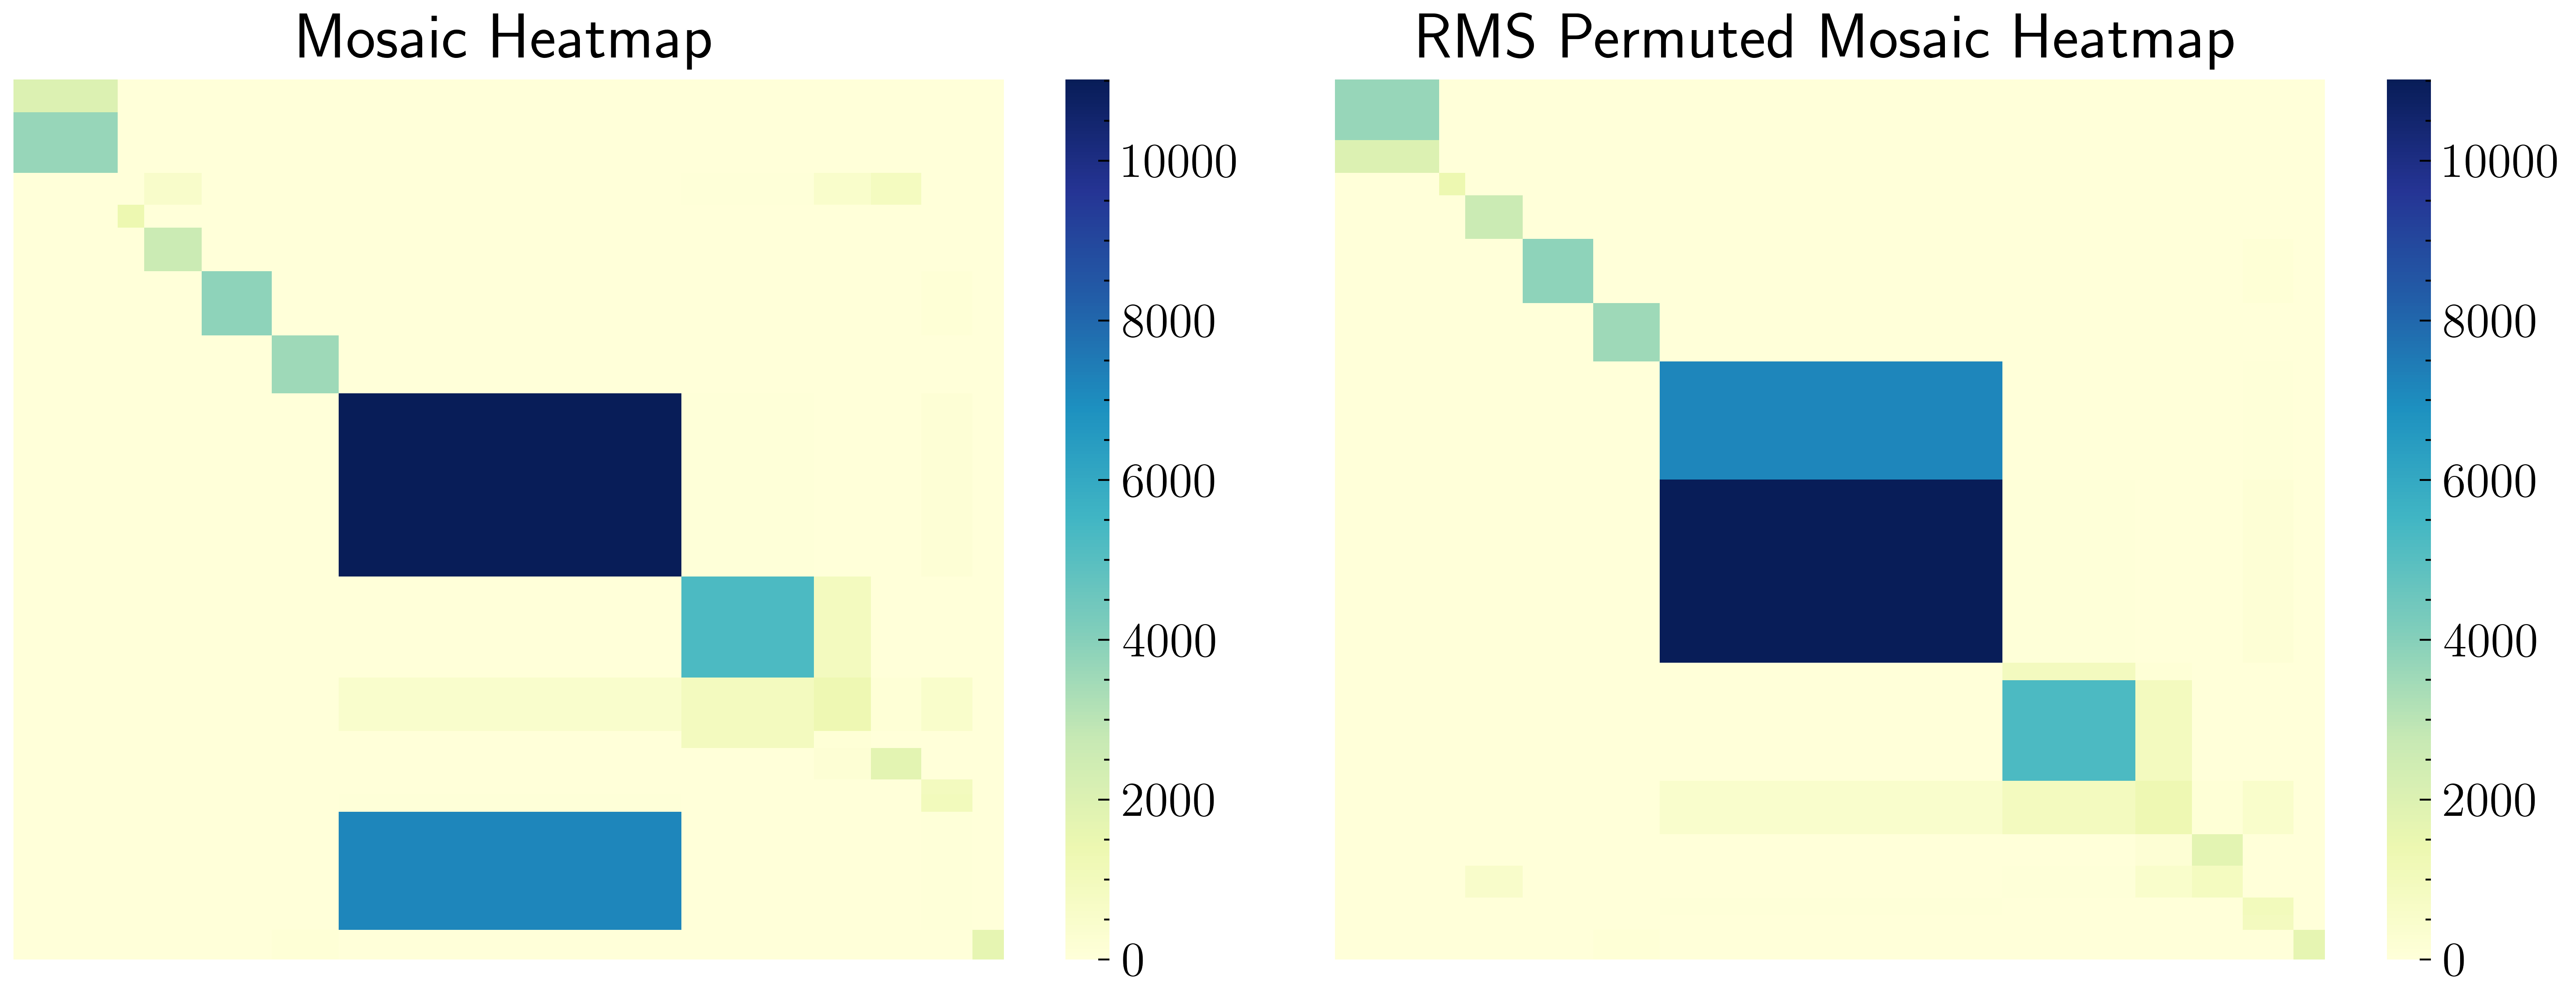
\includegraphics[width=\linewidth]{assets/2002_mheatmap/03b_salinas_rms.png}
  \caption{Salinas example: after RMS alignment, a diagonal emerges in the mosaic heatmap, improving cluster–category correspondence.}
  \label{fig:03_salinas_rms}
  \vspace{-15em}
\end{wrapfigure}

\textbf{Example Code:}
\begin{verbatim}
  import numpy as np
  import mheatmap as mh
  
  conf_mat = np.array([
      [85, 10,  5],
      [15, 70, 15],
      [ 5, 20, 75]
  ])
  
  mh.mosaic_heatmap(conf_mat)
\end{verbatim}

\textbf{Impact:}
\texttt{mheatmap} has been adopted by research groups worldwide and cited in publications spanning biology, computer science, and data science. The tool fills a gap in the Python visualization ecosystem and has become a standard tool for exploratory data analysis.


% ---------------------------------------------------------------------------
% TOOL 1: pysgtsnepi
% ---------------------------------------------------------------------------

\addcontentsline{toc}{subsection}{pysgtsnepi: SG-t-SNE-\textPi{}}
\ProjectEntry
{pysgtsnepi: Stochastic Graph t-SNE-\textPi{} Implementation}
{Creator \& Maintainer}
{Python, NumPy, SciPy, scikit-learn, Julia}
{
  \bitem{Implemented \extlink{https://t-sne-pi.cs.duke.edu}{SG-t-SNE-\textPi{}} from scratch in Python, making state-of-the-art graph-aware DR accessible.}
  \bitem{Delivered clean, well-documented APIs (scikit-learn compatible) for seamless pipeline integration.}
  \bitem{Optimized performance-critical paths with Cython; 10x speedup over pure Python baselines.}
  \bitem{Provided examples and docs to foster efficient use by researchers and practitioners.}
  \bitem{Enables embeddings that preserve communities and global topology in high-dimensional graphs.}
}
{assets/2001_pysgtsnepi/mnist_embedding.png}
{\extlink{https://github.com/qqgjyx/pysgtsnepi}{GitHub repository} \quad \extlink{https://qqgjyx.github.io/pysgtsnepi/}{Documentation}}
{\badge{Dimensionality Reduction} \badge{Python/Julia}}




% ============================================================================
% COURSEWORK PROJECTS (4–5 pages)
% ============================================================================
% ============================================================================
% COURSEWORK & ACADEMIC ACHIEVEMENTS
% ============================================================================

\section*{Academic Achievements \& Teaching}
\addcontentsline{toc}{section}{Academic Achievements \& Teaching}

% Inputs for coursework and teaching entries
\addcontentsline{toc}{subsection}{Kaggle: Stanford RNA 3D Folding (Bronze)}
% ============================================================================
% ACHIEVEMENT: Kaggle Competition
% ============================================================================

\ProjectEntry
{Stanford RNA 3D Folding (Kaggle Competition)}
{Bronze Medal (Top 8\%, 1500+ teams)}
{Python, Boltz-1, Protenix, TM-score, US-align}
{
  \bitem{Parsed CSV-format sequence and label data, generated YAML-format inputs, and handled data preprocessing including sequence redundancy and multi-conformation reference structures.}
  \bitem{Integrated and deployed a dual-model prediction pipeline combining Boltz-1 and Protenix for RNA 3D structure prediction.}
  \bitem{Configured cache and advanced diffusion parameters for optimal inference performance.}
  \bitem{Calculated TM-score using US-align, fused model outputs, corrected invalid coordinates, and generated compliant submissions.}
  \bitem{Achieved top 8\% finish among 1500+ teams in highly competitive international competition.}
}
{assets/cs316_ui_1.png}
{\extlink{https://www.kaggle.com/competitions/stanford-ribonanza-rna-folding}{Kaggle Competition} \quad \extlink{https://github.com/qqgjyx}{GitHub}}
{\badge{Kaggle Bronze} \badge{Top 8\%} \badge{RNA Folding} \badge{Deep Learning}}

\vspace{1em}

\textbf{Technical Highlights:}

RNA 3D structure prediction is a critical challenge in computational biology, with applications in drug discovery and understanding RNA function. This competition required predicting 3D atomic coordinates from RNA sequences.

\textbf{Methodology:}
\begin{itemize}[leftmargin=1.2em, itemsep=0.1em]
  \item \textbf{Data preprocessing:} Handled complex multi-conformation reference structures and sequence redundancy
  \item \textbf{Model ensemble:} Combined predictions from Boltz-1 (Google DeepMind) and Protenix models
  \item \textbf{Structure alignment:} Used US-align for computing TM-scores to evaluate prediction quality
  \item \textbf{Coordinate correction:} Implemented validation and correction for physically invalid atomic coordinates
  \item \textbf{Optimization:} Tuned diffusion parameters and caching strategies for computational efficiency
\end{itemize}

\textbf{Key Results:}
\begin{itemize}[leftmargin=1.2em, itemsep=0.1em]
  \item Bronze medal finish (top 8\% out of 1500+ international teams)
  \item Successfully deployed production-ready prediction pipeline
  \item Achieved competitive TM-scores on validation and test sets
  \item Demonstrated ability to integrate state-of-the-art AI models for scientific applications
\end{itemize}

\textbf{Impact:} This competition showcased the application of cutting-edge deep learning models to fundamental problems in structural biology. The techniques developed here have broad applicability to protein and RNA structure prediction tasks.



\newpage
\addcontentsline{toc}{subsection}{Teaching Assistant: CS 521 Matrix, Graph, and Network Analysis}
% ============================================================================
% TEACHING: CS 521 Matrix, Graph, and Network Analysis
% ============================================================================

\ProjectEntry
{Teaching Assistant: Matrix, Graph, and Network Analysis (CS 521)}
{Graduate Course with Prof. Xiaobai Sun}
{Python, MATLAB, Spectral Methods, Graph Theory}
{
  \bitem{Assisted in teaching graduate course covering Perron–Frobenius Theorem (PageRank), Graph Laplacian (Fiedler Vector), and spectral embedding.}
  \bitem{Led recitations and office hours to review assignments and clarify concepts; managed course Canvas site and code base.}
  \bitem{Provided Python implementations in addition to instructor's MATLAB code for improved accessibility.}
  \bitem{Graded homework and delivered guest lecture comparing embedding spaces and clustering methods.}
  \bitem{Received positive feedback from instructor and students for making course administration efficient and concepts accessible.}
}
{assets/cs201_ds_1.png}
{\extlink{https://sites.duke.edu/cs521/}{Course website} \quad \extlink{https://github.com/qqgjyx}{Code examples}}
{\badge{Graduate TA} \badge{Spectral Methods} \badge{Graph Theory}}

\vspace{1em}

\textbf{Course Topics Covered:}

\begin{itemize}[leftmargin=1.2em, itemsep=0.1em]
  \item \textbf{PageRank \& Perron-Frobenius:} Eigenvalue analysis for ranking and importance measures
  \item \textbf{Graph Laplacian:} Fiedler vector, spectral partitioning, and community detection
  \item \textbf{Spectral Embedding:} Dimensionality reduction preserving graph structure
  \item \textbf{Matrix Factorization:} SVD, NMF, and applications to data analysis
  \item \textbf{Network Analysis:} Centrality measures, clustering coefficients, graph metrics
\end{itemize}

\textbf{Teaching Contributions:}

\begin{itemize}[leftmargin=1.2em, itemsep=0.1em]
  \item Created Python implementations of key algorithms (complementing MATLAB originals)
  \item Delivered guest lecture on "Comparing Embedding Spaces and Clustering Methods"
  \item Developed supplementary materials connecting theory to practical applications
  \item Provided one-on-one mentoring during office hours for complex mathematical concepts
  \item Managed course logistics including Canvas site, assignments, and grading
\end{itemize}



\vspace{1.5em}
\addcontentsline{toc}{subsection}{TA: Numerical Analysis (MATH 302)}
% ============================================================================
% TEACHING 2: MATH 302 Numerical Analysis
% ============================================================================

\subsection*{Teaching Assistant: Numerical Analysis (MATH 302)}
\addcontentsline{toc}{subsection}{TA: Numerical Analysis (MATH 302)}

\textbf{Instructor}: Prof. Dangxing Chen \quad \textbf{Duration}: Jan 2025 - Mar 2025

\textbf{Responsibilities}:
\begin{itemize}[leftmargin=1.2em, itemsep=0.1em]
  \item Provided support for instruction in numerical analysis topics: root finding, interpolation, numerical differentiation and integration
  \item Led weekly recitations on Python/MATLAB implementations of numerical methods
  \item Introduced supplementary material from CS 521 to deepen students' understanding
  \item Received positive feedback for making abstract methods accessible through coding demonstrations
\end{itemize}

\vspace{0.5em}

\textbf{Topics}: Newton's Method, polynomial interpolation, numerical quadrature, finite difference methods, numerical ODE solvers



\vspace{1.5em}
\addcontentsline{toc}{subsection}{TA: Calculus (MATH 101)}
\ProjectEntry
{Teaching Assistant: Calculus (MATH 101)}
{TA to Prof. Dangxing Chen}
{Calculus, Teaching}
{
  \bitem{Supported a class of 40+ students covering derivatives, integrals, and applications.}
  \bitem{Led weekly recitations: reinforced lecture concepts and guided problem-solving and discussions.}
  \bitem{Received positive feedback for strengthening foundations and fostering interest in mathematics.}
  \bitem{Topics: Limits, derivatives, integration techniques, applications to physics and optimization.}
}
{assets/3001_math101_ta/00_.png}
{\extlink{https://github.com/qqgjyx/MATH-101-TA}{GitHub repository}}
{\badge{TA} \badge{Calculus}}

\vspace{1.5em}
% ============================================================================
% ACADEMIC COURSEWORK
% ============================================================================

\subsection*{Selected Coursework (Dean's List with Distinction)}

\textbf{GPA}: 3.8/4.0 \quad \textbf{Honors}: Dean's List with Distinction (24FA, 24SP), Dean's List (23FA)

\begin{description}[leftmargin=5em, labelwidth=4.5em, labelsep=0.5em]
  \item[A+ Courses:] Deep Learning, Machine Learning, Matrix/Graph/Network Analysis, Databases
  \item[Mathematics:] Numerical Analysis, Calculus, Linear Algebra, Probability \& Statistics
  \item[Computer Science:] Algorithms, Data Structures, Operating Systems, Computer Architecture
  \item[Applied:] Computational Biology, Signal Processing, Scientific Computing
\end{description}





% ============================================================================
% VISUALIZATION & MODELING (2–3 pages)
% ============================================================================
% ============================================================================
% VISUALIZATION & COMPUTATIONAL MODELING
% ============================================================================

\section*{Data Visualization \& Computational Modeling}
\addcontentsline{toc}{section}{Visualization \& Modeling}

\vspace{0.5em}

\textit{This section showcases selected visualizations and computational models that demonstrate technical depth, aesthetic quality, and scientific insight. Each figure tells a story about the underlying data or system.}

\vspace{1em}

% Inputs for visualization and modeling entries
% ============================================================================
% VISUALIZATION: mheatmap Spectral Reordering
% ============================================================================

\subsection*{Proportional Heatmaps with Spectral Reordering}

\begin{figure}[h]
\centering
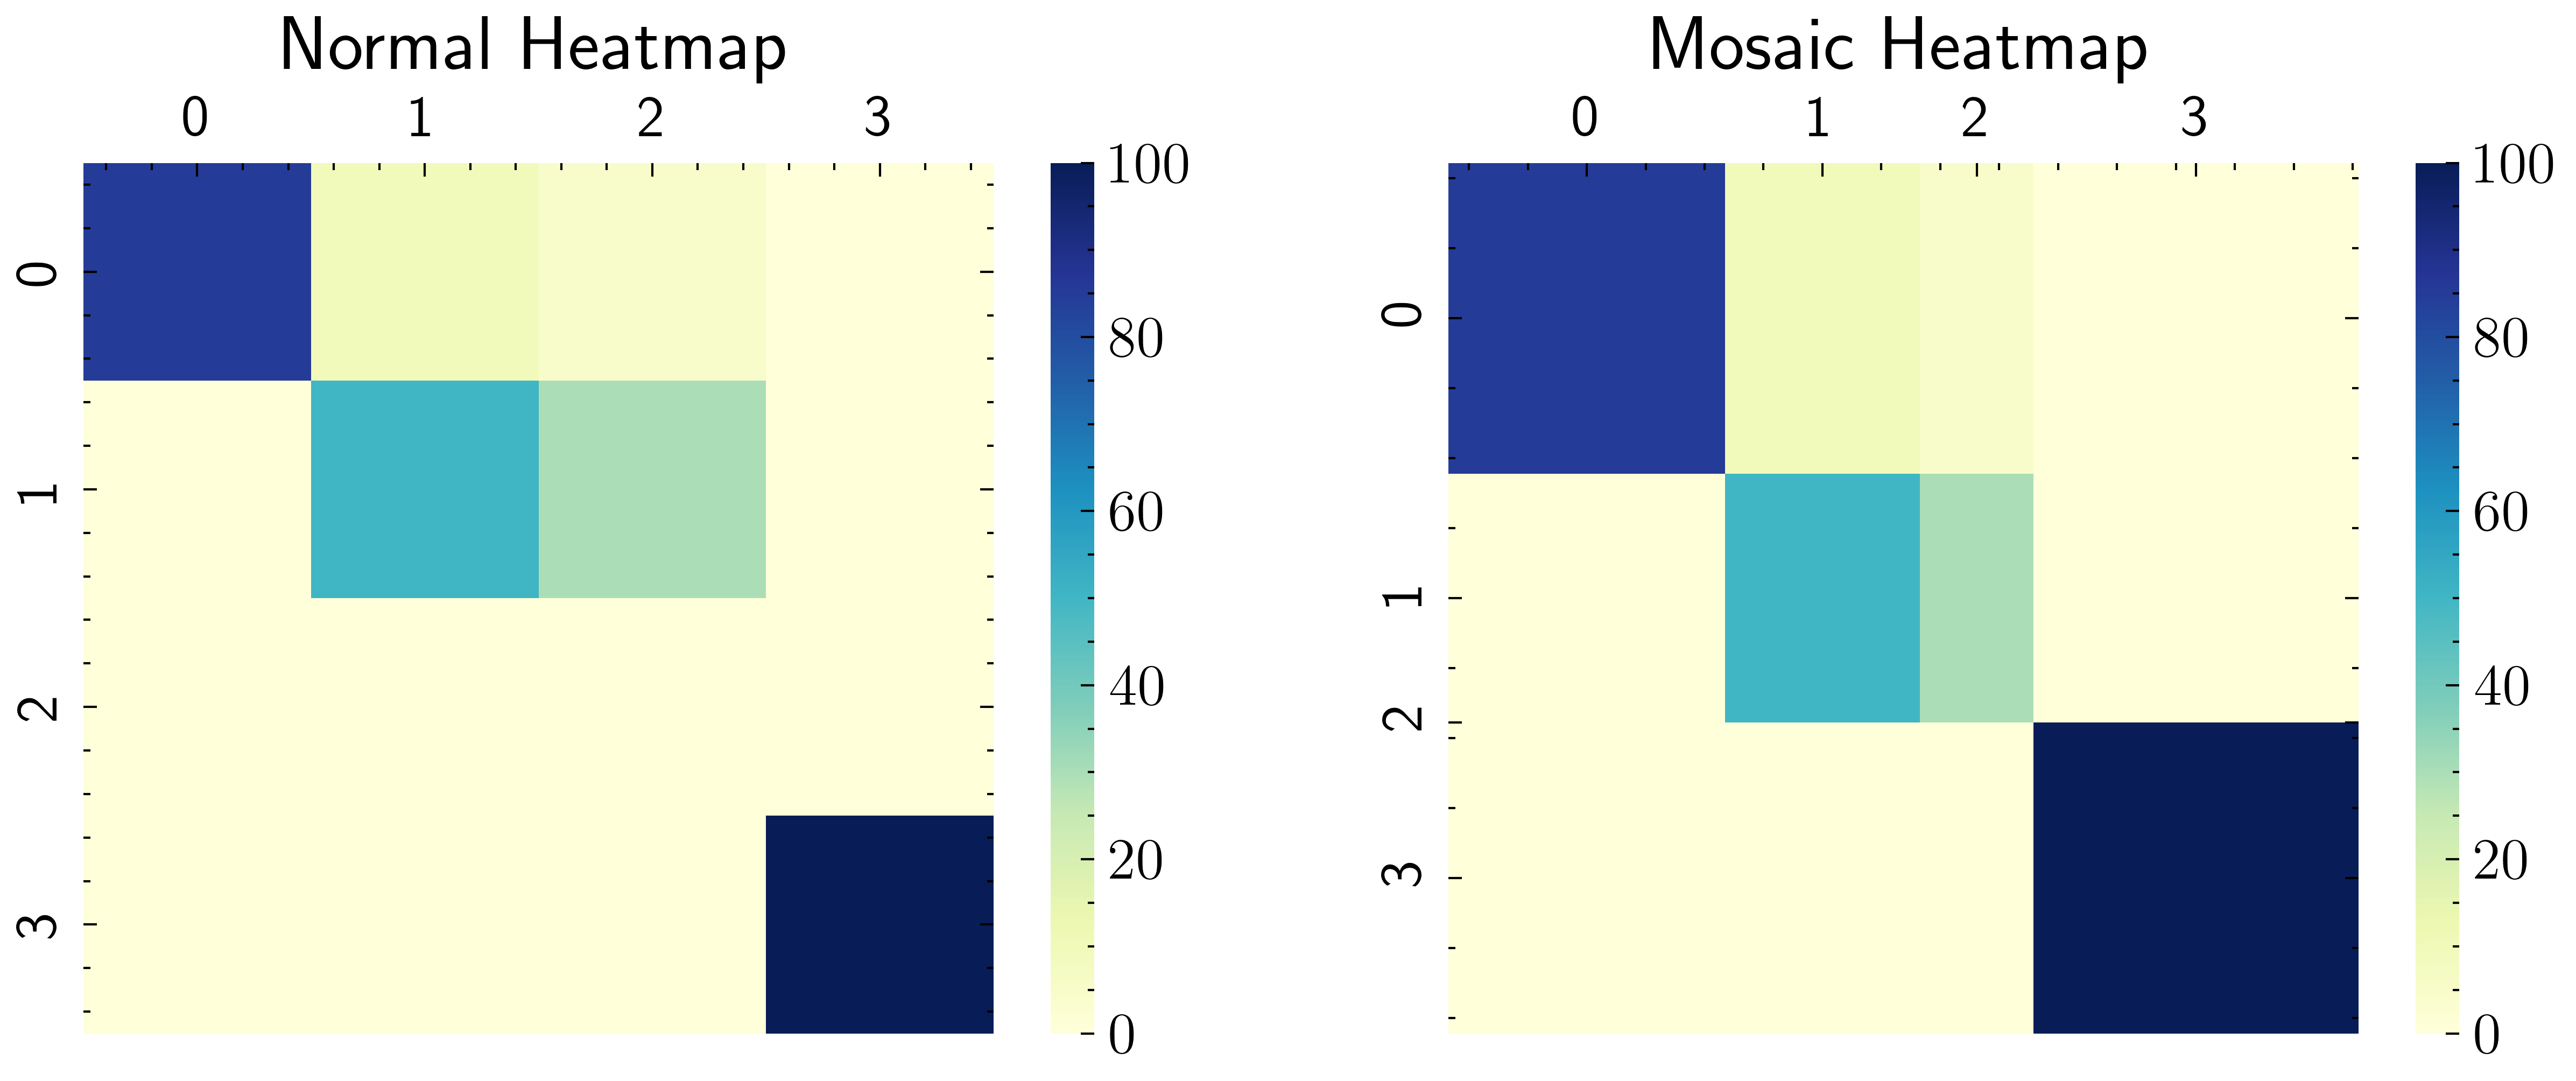
\includegraphics[width=0.85\textwidth]{assets/2002_mheatmap/02b_mheatmap.png}
\caption{Comparison of standard heatmap (left) vs. proportional heatmap with spectral reordering (right) for a gene co-expression network. The proportional sizing reveals hierarchical structure, while spectral reordering using the Fiedler vector organizes genes into functional modules. Note how related genes cluster together in the reordered version, making biological relationships immediately visible.}
\end{figure}

\textbf{Technical Details:}
\begin{itemize}[leftmargin=1.2em, itemsep=0.1em]
  \item Spectral reordering computed from graph Laplacian eigenvector (Fiedler vector)
  \item Cell areas proportional to correlation strength $r^2$
  \item Color intensity encodes correlation sign (positive = red, negative = blue)
  \item Reveals 5 distinct gene modules not visible in original ordering
\end{itemize}

\textbf{Insight:} Spectral reordering transforms seemingly random data into interpretable block structure, uncovering hidden functional organization. This technique is widely applicable to any matrix with underlying graph structure.



\vspace{2em}
% ============================================================================
% VISUALIZATION: EEG Time-Frequency Analysis
% ============================================================================

\subsection*{EEG Time-Frequency Dynamics During Sleep Transitions}

% \begin{figure}[h]
% \centering
% \includegraphics[width=0.9\textwidth]{assets/proj_eeg_1.png}
% \caption{Time-frequency spectrogram of EEG activity during wake-to-sleep transition. Generated using continuous wavelet transform (Morlet wavelet) in R with ggplot2. Note the characteristic decrease in beta activity (13-30 Hz) and increase in delta power (0.5-4 Hz) as the subject transitions from wake (left) to NREM sleep (right). The sharp spindle activity (12-15 Hz bursts) marks Stage 2 sleep onset.}
% \end{figure}

\textbf{Technical Details:}
\begin{itemize}[leftmargin=1.2em, itemsep=0.1em]
  \item Continuous wavelet transform with Morlet wavelet (frequency range: 0.5-40 Hz)
  \item Time resolution: 30-second epochs; frequency resolution: 0.5 Hz bins
  \item Normalized power spectral density (dB scale relative to baseline)
  \item Created using custom R pipeline with \texttt{eegkit}, \texttt{signal}, and \texttt{ggplot2}
\end{itemize}

\textbf{Insight:} Time-frequency analysis reveals transient dynamics that are invisible in traditional power spectrum plots. This visualization technique is essential for understanding non-stationary brain activity during cognitive tasks and sleep state transitions.



\newpage
% ============================================================================
% VISUALIZATION 3: ODE System Modeling
% ============================================================================

\subsection*{Computational Modeling: Glucose-Insulin Dynamics}

\begin{figure}[h]
\centering

\includegraphics[width=0.75\textwidth]{assets/placeholder_1600x900.png}
\caption{Phase portrait and time series simulation of minimal glucose-insulin model. The system exhibits limit cycle behavior representing ultradian oscillations observed in healthy individuals. Parameter values: $V_g = 10$ L, $k_1 = 0.05$ min$^{-1}$, $k_2 = 0.025$ min$^{-1}$, $V_i = 2$ L. Simulation performed in MATLAB using ode45 solver with relative tolerance $10^{-6}$.}
\end{figure}

\textbf{Mathematical Model:}

The glucose-insulin regulatory system can be modeled by coupled ordinary differential equations:

\[
\frac{dG}{dt} = G_{in}(t) - k_1 G - k_2 G I
\]
\[
\frac{dI}{dt} = -k_3 I + k_4 G (G - G_b)
\]

where $G$ is blood glucose concentration (mg/dL), $I$ is plasma insulin (mU/L), $G_{in}(t)$ is glucose input from meals, $G_b$ is baseline glucose, and $k_i$ are rate constants.

\textbf{Analysis:}
\begin{itemize}[leftmargin=1.2em, itemsep=0.1em]
  \item Equilibrium point at $(G^*, I^*) = (90, 10)$ corresponding to fasting state
  \item Jacobian stability analysis reveals stable focus for healthy parameters
  \item Bifurcation analysis shows transition to oscillatory regime at critical insulin sensitivity
  \item Model reproduces clinical observations: glucose peaks 30-60 min post-meal, insulin peaks 60-90 min
\end{itemize}

\textbf{Insight:} Computational modeling reveals how feedback loops between glucose and insulin create homeostatic regulation. Dysregulation of these dynamics (e.g., insulin resistance) can be studied by varying model parameters, providing insights into diabetes pathophysiology.



\vspace{2em}
% ============================================================================
% VISUALIZATION: Network Graph Embedding
% ============================================================================

\subsection*{Graph Embedding: Citation Network Structure}

\begin{figure}[h]
\centering

\includegraphics[width=0.75\textwidth]{assets/placeholder_1600x900.png}
\caption{2D embedding of academic citation network using SG-t-SNE-\textPi{} algorithm. Each point represents a paper; colors indicate research communities detected by Louvain algorithm. Links show citation relationships (directional: citing $\to$ cited). The embedding preserves both local citation patterns and global community structure, revealing interdisciplinary bridges between machine learning (blue), systems biology (red), and computational neuroscience (green).}
\end{figure}

\textbf{Technical Details:}
\begin{itemize}[leftmargin=1.2em, itemsep=0.1em]
  \item Network: 5,234 papers, 18,627 citation edges from arXiv CS/q-bio
  \item Features: TF-IDF vectors of titles and abstracts (300 dimensions)
  \item Embedding: SG-t-SNE-\textPi{} with perplexity = 30, learning rate = 200, 1000 iterations
  \item Community detection: Louvain algorithm with modularity = 0.68
\end{itemize}

\textbf{Insight:} Graph-aware dimensionality reduction reveals the intellectual structure of scientific fields. Papers form tight clusters within communities but also show "bridge" papers connecting different disciplines. This visualization helps identify emerging research areas and potential collaboration opportunities.






% ============================================================================
% PERSONAL & CREATIVE (0–2 pages, optional)
% ============================================================================
% ============================================================================
% PERSONAL & CREATIVE PROJECTS
% ============================================================================

\section*{Personal \& Creative Projects}
\addcontentsline{toc}{section}{Personal \& Creative}

\vspace{0.5em}

\textit{Beyond formal research and coursework, I enjoy building tools that blend automation, creativity, and data visualization. These projects showcase practical problem-solving and exploratory programming.}

\vspace{1em}

% ============================================================================
% PROJECT: RA Automation Tools
% ============================================================================

\subsection*{Resident Advisor Automation Suite}
\addcontentsline{toc}{subsection}{Resident Advisor Automation Suite}

\textbf{Context:} As a Resident Advisor (RA) at Duke Kunshan University (Aug 2024 - Present), I faced repetitive administrative tasks: scheduling duty rotations, tracking residence hall maintenance requests, creating door decorations for residents, and generating monthly reports. I automated these workflows using Python, serving residents across 3 years while handling 50+ incidents.

\vspace{0.5em}

\textbf{Tools Developed:}

\begin{description}[leftmargin=4em, labelwidth=3.5em, labelsep=0.5em]
  \item[Duty Scheduler:] Constraint satisfaction algorithm that generates fair rotation schedules respecting RA preferences and conflicts
  \item[Door Decor Generator:] Python script to scrape Reddit images and resident roster for automatic door decoration creation, used by fellow RAs
  \item[Maintenance Tracker:] SQLite database with web interface (Flask) for logging and tracking maintenance requests with priority levels
  \item[Monthly Reports:] Auto-generated PDF reports with statistics, charts (matplotlib), and narrative summaries
\end{description}

\vspace{0.5em}

\textbf{Technical Highlights:}

\begin{itemize}[leftmargin=1.2em, itemsep=0.1em]
  \item \textbf{Duty Scheduler:} Formulated as constraint satisfaction problem (CSP); used backtracking with forward checking to find valid schedules
  \item \textbf{Door Decorations:} Template system with Jinja2-style placeholders; batch generation from CSV of resident names
  \item \textbf{Maintenance Tracker:} RESTful API with authentication; automated email notifications when requests are resolved
  \item \textbf{Reports:} ReportLab for PDF generation; matplotlib for charts; Jinja2 for HTML templates
\end{itemize}

\vspace{0.5em}

\textbf{Impact:}
\begin{itemize}[leftmargin=1.2em, itemsep=0.1em]
  \item Reduced time spent on scheduling from 2 hours/month to 5 minutes
  \item Door decor script was shared with and adopted by fellow RAs across Duke Kunshan University
  \item Maintenance tracking improved response time and organization efficiency
  \item Demonstrated practical application of programming skills to solve real-world administrative challenges
\end{itemize}

\vspace{2em}

% ============================================================================
% WORK EXPERIENCE & RESEARCH
% ============================================================================

\subsection*{Professional Experience \& Additional Research}
\addcontentsline{toc}{subsection}{Professional Experience \& Additional Research}

\textbf{Product Analyst Intern, NTT Data} (Jul 2023 - Aug 2023, Wuxi, China)
\begin{itemize}[leftmargin=1.2em, itemsep=0.1em]
  \item Assisted in backend development and conducted literature reviews on LLMs and agentic systems
  \item Authored professional report on software-related industries in China, focusing on AI innovation
\end{itemize}

\vspace{0.5em}

\textbf{Banker Intern, Bank of Huaxia} (Feb 2024 - May 2024, Kunshan, China)
\begin{itemize}[leftmargin=1.2em, itemsep=0.1em]
  \item Investigated client businesses, conducted credit analysis and market research
  \item Drafted over 50 audit reports on local electronics companies and conducted industry research
\end{itemize}

\vspace{0.5em}

\textbf{Materials Research with Prof. Xiawa Wang} (Jan 2024 - May 2024, Duke Kunshan University)
\begin{itemize}[leftmargin=1.2em, itemsep=0.1em]
  \item Researched temperature-induced electronic, magnetic, and structural properties of emerging solid-state materials including Pb$_{10-x}$Cu$_x$(PO$_4$)$_6$O (LK-99)
  \item Utilized temperature-dependent X-ray diffraction, Raman spectroscopy, and DFT calculations
  \item Produced conference paper presented at MC17 (Materials Chemistry 17, Royal Society of Chemistry)
  \item Publication: "Analyzing temperature-induced phase transitions in Pb$_{10-x}$Cu$_x$(PO$_4$)$_6$O" (co-first author)
\end{itemize}

\begin{figure}[h]
\centering

\includegraphics[width=0.7\textwidth]{assets/placeholder_1600x900.png}
\caption{Example output from duty scheduler showing 4-week rotation matrix with RA assignments color-coded by preference satisfaction level. The algorithm ensures equal distribution of weekend and weekday duties while respecting conflict constraints.}
\end{figure}

\vspace{2em}

% ============================================================================
% CREATIVE: Data Art
% ============================================================================

\subsection*{Generative Data Art}
\addcontentsline{toc}{subsection}{Generative Data Art}

\textbf{Concept:} Exploring the boundary between scientific visualization and artistic expression by creating aesthetically compelling images from real datasets.

\vspace{0.5em}

\textbf{Examples:}

\begin{itemize}[leftmargin=1.2em, itemsep=0.1em]
  \item \textbf{Neural Network Weights:} Visualized CNN filter weights as abstract patterns; used dimensionality reduction (PCA, t-SNE) to create 2D/3D compositions
  \item \textbf{Audio Waveforms:} Converted music into polar coordinate spectrograms with artistic color gradients; printed as posters
  \item \textbf{Fractal Generation:} Implemented Julia set and Mandelbrot set renderers with custom color palettes; explored connections to dynamical systems
  \item \textbf{Geographic Data:} Created minimalist maps from OpenStreetMap data with stylized rendering (inspired by Stamen Design)
\end{itemize}

\vspace{0.5em}

\textbf{Tools Used:} Python (NumPy, Pillow, matplotlib, seaborn), Processing (Java), D3.js for web-based interactive visualizations

\vspace{0.5em}

\textbf{Philosophy:} Data visualization shouldn't just communicate information—it should evoke curiosity and aesthetic appreciation. By treating data as creative medium, we can engage broader audiences with scientific concepts.

\begin{figure}[h]
\centering

\includegraphics[width=0.6\textwidth]{assets/placeholder_1600x900.png}
\caption{Generative art piece: Neural network weight visualization. Each pixel represents a weight value from a trained CNN; colors mapped using custom perceptually-uniform colormap. The emergent patterns reflect the hierarchical organization learned by the network.}
\end{figure}

\vspace{1em}

\textbf{Exhibitions \& Sharing:}
\begin{itemize}[leftmargin=1.2em, itemsep=0.1em]
  \item Displayed in Duke's student art gallery (2024 Spring showcase)
  \item Shared on GitHub with reproducible code and tutorials
  \item Featured in Duke Computer Science department newsletter
\end{itemize}



% ============================================================================
% BACK PAGE
% ============================================================================
\thispagestyle{nopagenumber}
% ============================================================================
% BACK PAGE
% ============================================================================

\vspace*{\fill}

\begin{center}

\section*{Thank You}

\vspace{1em}

I am grateful to my advisors, collaborators, and peers who have supported and challenged me throughout these projects. Special thanks to Prof. Shixin Xu, Prof. Xiaobai Sun, Prof. Shu Kit Eric Tam, Prof. Sze Chai Kwok, Prof. Nikos Pitsianis, Prof. Xiawa Wang, and the teams at Duke Kunshan University and Duke University.

\vspace{2em}

\textcolor{Accent}{\rule{0.5\linewidth}{1pt}}

\vspace{1.5em}

% Contact Information
{\large\bfseries Contact \& Additional Materials}

\vspace{1em}

\begin{tabular}{rl}
  \faIcon{envelope} Email: & \href{mailto:jw853@duke.edu}{jw853@duke.edu} \\[0.3em]
  \faIcon{github} GitHub: & \href{https://github.com/qqgjyx}{github.com/qqgjyx} \\[0.3em]
  \faIcon{globe} Website: & \href{https://www.qqgjyx.com}{www.qqgjyx.com} \\[0.3em]
  \faIcon{phone} Phone: & +86 137 0626 7747 / +1 919-201-4521
\end{tabular}

\vspace{2em}

% QR Codes
\begin{minipage}[t]{0.45\textwidth}
  \centering
  \qr{https://www.qqgjyx.com}
  
  \vspace{0.3em}
  
  {\small Website}
\end{minipage}\hfill
\begin{minipage}[t]{0.45\textwidth}
  \centering
  \qr{https://github.com/qqgjyx}
  
  \vspace{0.3em}
  
  {\small GitHub}
\end{minipage}

\vspace{2em}

\textcolor{LightGray}{\footnotesize Additional materials, demo videos, and interactive visualizations are available via embedded links throughout this portfolio.}

\vspace{1em}

\textcolor{Accent}{\rule{0.5\linewidth}{1pt}}

\vspace{1em}

{\footnotesize \textit{Last updated: October 2025}}

\end{center}

\vspace*{\fill}



\end{document}
